\documentclass[12pt,a4paper,oneside]{book} % twoside for draft

\usepackage{hyperref}
%\usepackage{babel}
\usepackage[utf8]{vietnam}
\usepackage[english]{babel}
%\usepackage{times}
%\usepackage{graphicx}
\usepackage{tabularray}
\usepackage{mathptmx}	% same Time New Roma
%\renewcommand{\rmdefault}{phv} % Arial
%\renewcommand{\sfdefault}{phv} % Arial
\usepackage{longtable}
\usepackage{fancyhdr}
\usepackage{algorithm2e}
\usepackage{graphicx}
\usepackage{float}
\usepackage{bkthesis}


% \csdeptname{KHOA ĐIỆN ĐIỆN TỬ}
\crname{CAPSTONE PROJECT REPORT}
% \crname{BÁO CÁO TIỂU LUẬN}
\title{PETOPIA - A PET ADOPTION PLATFORM}
\cstuname{STUDENT 1: BUI NGOC DUC ANH (2052832)
\\STUDENT 2:	NGUYEN MINH HUNG	(2052504)
\\STUDENT 3:	HUYNH VO TUAN	(2053558)}


\csCouncil{COMPUTER SCIENCE}
\csSupervise{TRUONG TUAN ANH, Ph.D.}
\csReviewer{MAI DUC TRUNG, M.Eng.}
\cttime{6/2024}

\thesislayout

\begin{document}
%-	Bìa cứng - màu xanh dương, chữ mạ vàng (xem mẫu đính kèm)
%-	Trang tên (tờ lót): chất liệu giấy, nội dung giống như bìa LV
%-	Ở gáy LV: in nhan đề LV (có thể in tóm tắt nếu nhan đề quá dài), size 15 – 17
%-	Phiếu Nhiệm vụ LV, chấm điểm Hướng dẫn & Phản biện (đã ký): nhận từ GVHD & GVPB sau khi bảo vệ (theo lịch hẹn).
%-	Lời cam đoan
%-	Lời cảm ơn/ Lời ngỏ
%-	Tóm tắt LV
%-	Mục lục
%-	Danh mục, bảng biểu, hình ảnh, ... (nếu có)
%-	Nội dung LV
%-	Danh mục TL tham khảo
%-	Phụ lục (nếu có)

\coverpage

\frontmatter

% add content here
%-	Lời cảm ơn/ Lời ngỏ
\begin{acknowledgment}
	To complete this specialized project, we express deep gratitude to Prof. Truong Tuan Anh for his dedicated guidance throughout the research process. We sincerely thank the professors in the Faculty of Computer Science and Engineering at Ho Chi Minh City University of Technology for imparting knowledge during our years of study at the university. The accumulated knowledge acquired during our academic journey not only forms the foundation for our research but also serves as a confident stepping stone into the future.

Finally, we wish the esteemed professors abundant health and success in their noble careers.

\end{acknowledgment}


%-	Lời cam đoan
\begin{commitment}
	We guarantee that this project, which includes a report and a software system, is our own and conducted under the supervision and guidance of Prof. Truong Tuan Anh. The result of our research is legitimate and has not been published in any form before this. All materials used within this research are collected by ourselves, from various sources, and are appropriately listed in the references section. In addition, within this research, we also used the results of several other authors and organizations. They have all been aptly referenced. In any case of plagiarism, we stand by our actions and are to be responsible for it. Ho Chi Minh City University of Technology, therefore, is not responsible for any copyright infringements conducted within our research.
\end{commitment}


%-	Tóm tắt LV
\begin{abstract}
	The “Petopia - Pet Adoption Platform” project is a comprehensive initiative aimed at improving the process of pet adoption. This online platform serves as a bridge, connecting potential pet adopters with animal shelters and rescue groups in Ho Chi Minh City. The primary goal is to streamline the adoption process, making it easier for people to find their perfect pet companion and also creating a hub where pet enthusiasts can access information and gain knowledge about pet care.

The platform provides detailed profiles of each pet available for adoption. This allows potential adopters to gain a thorough understanding of the pet. One of the key features of the platform is its advanced search functionality. Users can search for pets based on various criteria such as breed, size, age, and pictures with the support of AI technology. This feature is designed to help users find a pet that fits their lifestyle and preferences, thereby increasing the rate of successful adoption.

In addition, the platform also offers a wealth of resources for pet lovers. These resources cover a wide range of topics, from the adoption process itself to pet care tips and advice. The aim is to equip new pet owners with the knowledge they need to provide their new pets with a loving and caring home.

In conclusion, by applying the knowledge of programming and software engineering, this capstone project hopes to create a solution that benefits both animals in need and potential pet owners. It aims to reduce the number of animals in shelters and rescue groups by increasing the rate of successful adoptions. At the same time, it seeks to bring joy and companionship to families and individuals looking to adopt a pet.

\end{abstract}

\tableofcontents
%\listofsymbols
\listoftables


\listoffigures
%\listofalgorithms


\mainmatter

\fancyhead{}  % Clears all page headers and footers
%\rhead{\thepage}  % Sets the right side header to show the page number
%\lhead{}  % Clears the left side page header
%\fancyfoot[positions]{footer}
\renewcommand{\footrulewidth}{0.4pt}

\pagestyle{fancy}  % Finally, use the "fancy" page style to implement the FancyHdr headers


\chapter{INTRODUCTION}
\section{Context}
In recent years, Vietnam, and Ho Chi Minh City, in particular, have seen a significant surge in the demand for pet adoption. This growing trend underscores the increasing necessity for organizations involved in pet adoption to enhance their systems and operational procedures. This will ensure they can effectively meet the escalating demand and continue to provide excellent service to those seeking to adopt pets.

Established in 2015, Saigon Time (SGT) has earned a reputation as one of the leading stray pet organizations in Ho Chi Minh City. The organization has been instrumental in providing care and treatment for numerous abandoned dogs and cats, successfully finding them new homes. Like many pet rescue and adoption organizations in the city, SGT primarily operates through a Facebook fan page. Recognizing the need for more effective management and a professional pet adoption process, as well as the desire to expand the organization’s operations, SGT has decided to develop a dedicated software system.

\section{Problems}

As previously noted, Saigon Time operates exclusively on Facebook. However, with the growing user base and the organization’s desire to expand its operational capabilities, several challenges have emerged:
\begin{itemize}
    \item \textbf{User Experience}: Users are finding it difficult to search for and identify suitable pets for adoption. The current process does not effectively accommodate the extensive information about each pet that needs to be considered before adoption.
    \item \textbf{Pet Giving Process}: Currently, the pets in SGT’s system are those physically present at their operating location. In the future, SGT aims to allow individuals wishing to give their pets to proactively post about their pets for adoption. This development necessitates the implementation of a system capable of managing the adoption process between users.
    \item \textbf{System Management}: The increasing number of users and pets has made it challenging for SGT administrators to manage the system. Information such as the number of pets, number of users, etc., is currently managed using office tools. This situation underscores the need for a centralized management solution for pet posting, adoption, data management, and system operations.
\end{itemize}

\section{Goals}

A software system can serve as a solution to the mentioned issues by establishing a platform that bridges the gap between pet shelters, rescues, pet owners, and potential adopters. This system can be tailored to assist individuals in finding pets that align with their preferences and lifestyle, offering insights into the pet’s health, temperament, and background. It can also simplify the adoption process by enabling users to submit adoption applications online, schedule appointments to meet pets, and finalize the adoption process digitally.

Furthermore, the software system can enhance the efficiency of SGT administrators in managing their operations. It can offer tools for handling pet records, monitoring adoptions, and tracking system usage. Additionally, it can assist shelters, rescues, and other businesses in promoting their services.

Lastly, the system is designed to transform SGT into a hub where pet enthusiasts can access information and gain knowledge about pet care.

\section{Scope}

This specialized project aims to develop a comprehensive software system that will streamline the operations of the SGT organization, moving away from its current reliance on a Facebook page. The proposed software system will consist of:
\begin{itemize}
    \item A web application for users who are interested in adopting or giving away pets, as well as for organizations that wish to collaborate with SGT.
    \item	A web application specifically designed for SGT administrators to effectively manage the entire system.
    \item Supporting programs and services to ensure the accuracy and seamless operation of the aforementioned applications.
\end{itemize}

\section{Report structure}
Our specialized project report will be structured into the following chapters:
\begin{enumerate}
    \item \textbf{Introduction}: This chapter will provide essential background information on the project topic and clearly state the project’s objectives.
    \item \textbf{System Analysis}:  This chapter will concentrate on the collection and analysis of business requirements. It will employ a range of techniques to translate these requirements from a common language into a format suitable for system design and implementation.
    \item \textbf{System Design}: This chapter will present detailed designs and methodologies to fulfill the requirements established in the system analysis phase.
    \item \textbf{Technologies}: Introducing the technologies, frameworks, and main libraries used to implement the project.
    \item \textbf{System Implementation}: Outlining the process involved in implementing the system functions, this chapter provides a comprehensive view of how the system was brought to life.
    \item \textbf{System Testing}:  Covering essential aspects related to testing the functionality and performance of your project.
    \item \textbf{Deployment Plan}: Describing the steps needed to successfully introduce our project to end users.
    \item \textbf{Conclusions and Future plan}:  Summarizing the project, this chapter will discuss contributions, limitations, weaknesses, and recommendations for future research.
\end{enumerate}


Each chapter aims to provide a thorough exploration of its respective topic, ensuring a comprehensive understanding of the project.

\chapter{SYSTEM ANAYLYSIS}
\section{Market Survey}
To comprehend the scope and orientation of the system, it’s essential to conduct a market survey of similar systems. Pet adoption systems, each with its unique features and benefits, come in various forms. In Vietnam, however, most organizations in this field operate through social network pages like Facebook and Instagram, rather than standalone software systems. Notably, the only pet adoption system that stands out from the rest is Hanoi Pet Adoption, which warrants further analysis and evaluation.

\subsection{Overview}
The Hanoi Pet Adoption (HPA) system, a web application based in Hanoi, Vietnam, serves as a platform for individuals to find and adopt rescued animals. The primary objective of this system is to aid the HPA group in rescuing and caring for animals, and subsequently finding them loving and responsible homes.

HPA has the following main features:
\begin{itemize}
    \item \textit{Pet profiles:} The system showcases profiles of animals ready for adoption. These profiles include details such as photos, names, genders, ages, colors, and sterilization statuses.
    \item \textit{User Preferences:} Users can filter animals based on their preferences, including gender, age, color, and sterilization status.
    \item \textit{Volunteer Contact Information:} The system provides the contact information of volunteers responsible for each animal, enabling users to inquire further about their animal of interest.
    \item \textit{Adoption Process Guidance:} The system guides users through the adoption process, which includes an interview, a contract, and a fee.
\end{itemize}

\subsection{Evaluation}
HPA provides a comprehensive and effective pet adoption support process. However, its limitation lies in its exclusivity - only system administrators of the organization are permitted to post pet profiles onto the system.

The absence of a messaging system in the current platform can create challenges in the pet adoption process. This lack of direct communication makes it difficult for system administrators and users to contact each other, particularly when issues arise. A messaging system would facilitate smoother interactions and problem resolution, enhancing the overall user experience.

Currently, the system requires manual input for posting, filtering, and searching functions. This can pose challenges for individual users, potentially reducing the efficiency of posting and searching, and negatively impacting the user experience.

Lastly, a significant feature that is absent in the system is a notification system. Such a system would alert users when pets that meet their criteria are posted, ensuring that users are promptly informed about potential matches. This feature could greatly enhance the user experience and effectiveness of the pet adoption process.

\subsection{Potential Improvements}
After a thorough review of the strengths and weaknesses of existing systems, we have identified several potential enhancements that could significantly improve the user experience and functionality of the system.

Firstly, we propose to \textbf{expand the HPA system}. Currently, the pets are only posted by system administrators. However, SGT aims to allow individuals wishing to surrender their pets to proactively post about their pets for adoption. This expansion would not only increase the number of pets available for adoption but also provide a platform for pet owners and organizations to share valuable information and updates about their pets.

Secondly, we suggest the implementation of \textbf{interactive pet profiles}. This feature would allow users to visit and interact with pet profiles and posts. This interaction could include liking, commenting, or sharing a pet’s profile.

Next, we recommend \textbf{applying Artificial Intelligence (AI) technology to enhance the posting and searching} functionality of the system. With this feature, users could simply upload a pet image, and the AI would automatically populate most of the input fields, such as breed, and color. This would not only simplify the process of posting a pet profile but also increase the accuracy and consistency of the pet information in the system.

In addition, we propose the implementation of a \textbf{notification system}. This system would alert users when a pet that matches their preferences becomes available on the system. User criteria for filtering pet profiles(such as breed, age, or size) will be referenced, and then users can receive notifications when a matching pet is posted. This would ensure that users don’t miss out on potential matches and can act quickly to adopt their desired pet.

Lastly, we suggest establishing a \textbf{messaging system} that facilitates communication among pet adopters, pet owners, and system administrators. This system would allow users to ask questions, clarify information, or arrange meetings, enhancing the overall user experience and streamlining the adoption process. By providing a platform for direct communication, we can foster a sense of community among users and promote open and transparent discussions about pet adoption.

In conclusion, these enhancements aim to make the system more user-friendly, efficient, and effective in connecting pets with potential adopters. We believe that by implementing these changes, we can take a significant step toward our goal of finding a loving and suitable home for every pet.

\section{Stakeholders}
Stakeholders for a project focused on creating a pet adoption platform in Vietnam would include a diverse range of individuals, organizations, and groups with an interest in or influence over the project. Here are some key stakeholders:
\begin{itemize}
    \item \textit{Administrator:} The administrator is responsible for managing and overseeing the platform's operations. They have control over user accounts, content moderation, and the overall functionality of the website.
    \item \textit{Pet Adopter:} Pet adopters are individuals looking to provide a loving home to pets available for adoption. They may already own pets or be first-time pet owners. Pet adopters interact with pet owners and adoption agencies through messaging and inquiries about available pets. They can also share their adoption stories and experiences with the platform's community.
    \item \textit{Pet Owner:} Pet owners are individuals who currently own and care for pets, including dogs, cats, or other animals. Or those, for various reasons, have decided to give their pets to new homes. Reasons may include relocation, financial constraints, allergies, or changes in life circumstances.
    \item \textit{Guest:} Guests are individuals who visit the platform without creating an account or logging in. They have limited access to platform features and content. Guests can browse public content, view pet listings, read provided blogs, and explore the platform's resources. They can also choose to create an account to access more features.
    \item \textit{Pet Adoption Agencies and Shelters:} Organizations involved in pet adoption, rescue, and rehoming would benefit from the platform as it could help them find suitable homes for abandoned or rescued animals. They might also contribute content and listings.
    \item \textit{Pet-Related Businesses:} Pet stores, pet food suppliers, grooming salons, veterinary clinics, and other businesses in the pet industry have a stake in the project. They could use the platform to advertise their products and services to a targeted audience.
    \item \textit{Veterinarians:} Veterinarians play a crucial role in pet healthcare. They might use the platform to provide information, answer questions, and offer telehealth services. Their expertise can be valuable to pet owners.
    \item \textit{Investors and Funders:} Individuals or organizations providing funding or investment for the development and scaling of the platform are stakeholders with a financial interest.
\end{itemize}

Understanding and engaging with these stakeholders will be important for the success and sustainability of the project. Each stakeholder group may have different needs, interests, and concerns that should be addressed during the project's planning and execution.

\section{Requirements eliciation}
\subsection{Functional Requirements}


\begin{table}
    \centering
    \begin{tblr}{
            vline{1-3} = {-}{},
            hline{-} = {1-2}{},
        }
        \textbf{Group}                                    & \textbf{Requirements} &   & \\
        \textbf{Authentication and authorization}         & {
                -~~~~~~~
                Users can create new accounts by providing personal information.
        \\-~~~~~~~
                Users can log into the system using Google accounts.
        \\-~~~~~~~
                Users can log into the~ system by
                providing a registered email and password.
        \\-~~~~~~~
                Users can send applications to the system to update their accounts to
                Organization accounts.
        \\-~~~~~~~
                Admins can verify Organizations’ registration and upgrade users’
                accounts.
        \\-~~~~~~~
                Users can reset or recover their account passwords.
        }                                                 &                       &     \\
        \textbf{Pet profile management}                   & {
                -~~~~~~~
                Users can create pet profiles by giving details such as name, species,
                breed, age, color, health status, sterilization status, pictures, and videos
                of pets.
        \\-~~~~~~~
                Users can provide information about breed, species, and color by
                uploading pets’ pictures.
        \\-~~~~~~~
                Pet photos and text inputs must be sensitive-validated before
                uploading.
        \\-~~~~~~~
                Users can edit their pet profiles.
        \\-~~~~~~~
                Users can publish, hide, or remove their pet profiles.
        \\-~~~~~~~
                Admins can remove or hide any pet profiles of the system.
        }                                                 &                       &     \\
        \textbf{Pet profile filter and view}              & {
                -~~~~~~~
                Users can search for pets by providing filtering options such as name,
                species, breed, age, color, health status, and sterilization status.
        \\-~~~~~~~
                Users can search for pets by providing pets’ pictures.
        \\-~~~~~~~
                Users can view pet profiles with detailed information such as name,
                species, breed, age, color, health status, sterilization status, pictures,
                and videos of pets
        }                                                 &                       &     \\
        \textbf{Pet adoption}                             & {
                -~~~~~~~
                Users can submit applications to adopt pets on the system.
        \\-~~~~~~~
                Users can view, decline, or accept adoption applications sent to their
                pets.
        }                                                 &                       &     \\
        \textbf{User interaction and engagement}          & {-~~~~~~~
                Pet
                Adopters can send messages to Pet Owners, Organizations, and Admins.
        \\-~~~~~~~PetAdopters have to update their pets’ status every seven days[1]~ from the date they received the petsby uploading posts in the adopt status section of the pet profile.\\-~~~~~~~
                Pet
                Adopters can set their posts public for all users or just Admins, and Pet
                Owners.
        \\-~~~~~~~
                Admins
                and Pet Owners can view and interact with posts from Pet Adopters.
                All users of the system can view and interact
                with posts from Pet Adopters if the posts are public.
        \\~ ~ ~ ~ ~ ~~}       &                       &     \\
        \textbf{Blog management}                          & {
                -~~~~~~~
                Admins and Organizations can create and publish blogs.
        \\-~~~~~~~
                Organizations can apply advertisements on their blogs.
        \\-~~~~~~~
                Organizations can edit or remove their blogs.
        \\-~~~~~~~
                Admins can hide or remove any blogs of the system.
        }                                                 &                       &     \\
        \textbf{Advertisement and payment}                & {
                -~~~~~~~
                Organizations can choose advertisement duration with different prices.
        \\-~~~~~~~
                Organizations can pay advertisement fees through an online banking
                service.
        \\-~~~~~~~
                Admins can receive advertisement fees through an online banking
                service.
        \\-~~~~~~~
                System provides admins and organizations information like payment
                status and invoices.
        }                                                 &                       &     \\
        \textbf{Notifications}                            & {
                -~~~~~~~
                Users can receive notifications on new pet adoption applications.
        \\-~~~~~~~
                Users can receive notifications on new pets’ status posts uploaded.
        \\-~~~~~~~
                Users can receive notifications on new pet profiles matching their
                criteria.
        }                                                 &                       &     \\
        \textbf{System statistics for administrators}     & -~~~~~~~
        Admins can get statistics about systems usages, such as the number of
        pet profiles, adopted pets; number of users and Organizations; number of
        blogs, and the total amount of advertisement fee. &                       &
    \end{tblr}
\end{table}

\chapter{SYSTEM DESIGN}

\section{System architecture}
With the completion of system analysis, we are now 
focusing on designing the system architecture, how the system is organized and served to the end users. This section will 
discuss the detailed system architecture and services for deploying the system. As we 
can see from \textit{Figure 3.1}, the proposed architecture contains the 
following components:
\begin{figure}[H]
    \centering
    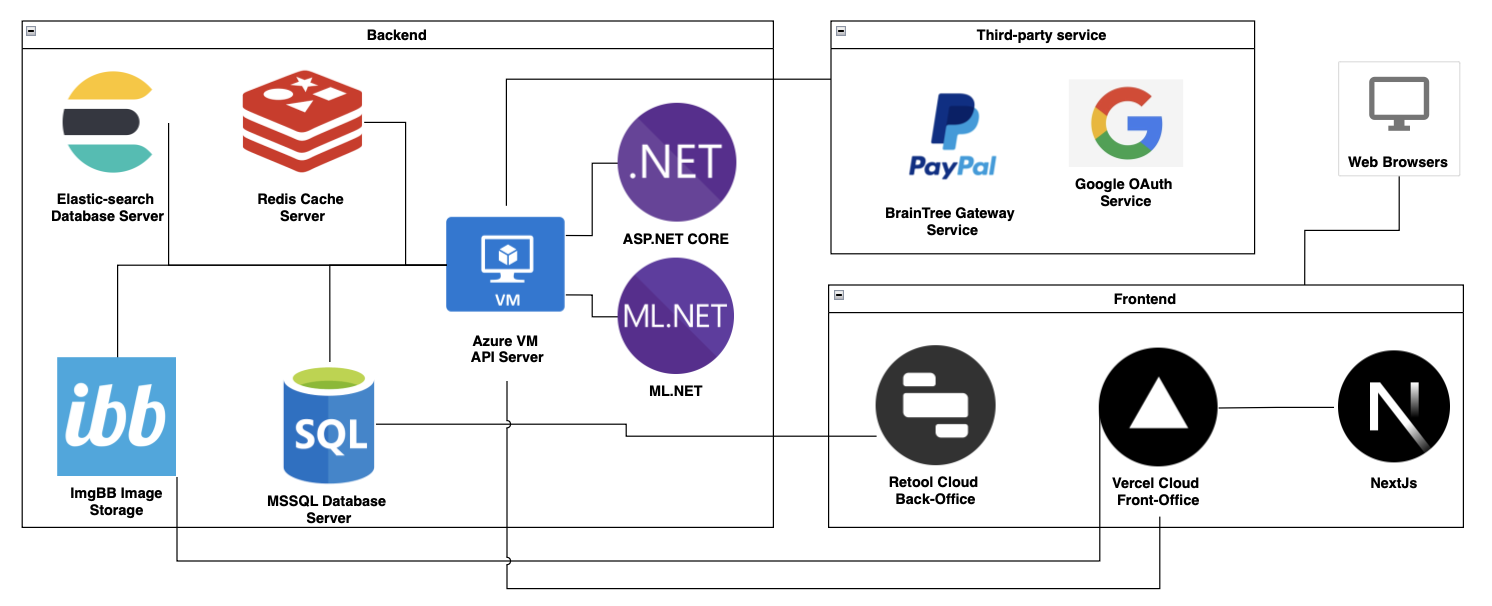
\includegraphics[width=1\textwidth]{Figures/Deployment/architect-report.png}
    \caption{Architecture Diagram}
    \label{fig:deployment-architecture}
\end{figure}
The Frontend component contains the back office and front office website of the system. This component is served to end users through web browsers.
\begin{itemize}
    \item \textit{Front office} handles user events and calls restful APIs from the API Server. It is implemented using Next.js and deployed on Vercel.
    \item \textit{Back office} is implemented using Retool. It interact directly to the MSSQL Database Server.
\end{itemize}

The backend of the system includes components as follows:
\begin{itemize}
    \item \textit{API Server} is the central part of the system, focusing on 
    handling all business logics and flows, serving API for the front office, 
    and interacting with other components of the system. It is implemented by ASP.NET Core and ML.NET and deployed by an Azure Virtual Machine.
    \item \textit{MSSQL Database Server} is the place where the database of the system is served. 
    This server interacts with the API Server and the back office.
    \item \textit{Imgbb Image Server} stores all the static images of the system. Images will 
    be uploaded directly from the front office to the Imgbb Image Server before storing the returned URLs in the SQL Database Server. This component will 
    be served by a free Imgbb cloud service.
    \item Furthermore, we will have two corresponding servers for caching data and optimizing 
    data search speed using a free \textit{Elastic-search cloud} and \textit{Azure Redis Cache Database}.
\end{itemize}

Finally, third-party services for authentication (Google OAuth Service) and payment (BrainTree Gateway Service) purposes are implemented by connecting to the API Server.

\section{UI/UX design}

In this section, we delve into the UI/UX design for our pet adoption website. Each page has been crafted to enhance user engagement and streamline the adoption process. Begins on the homepage, where users are welcomed with an intuitive interface that serves as the gateway to the platform. The login and register pages provide a seamless onboarding experience, ensuring a secure and personalized environment. The pet search page facilitates effortless exploration, allowing users to discover potential companions with ease. Detailed pet profiles showcase comprehensive information, fostering informed decision-making. The user profile page ensures a tailored experience, while the blog homepage and pages provide valuable insights and updates. To navigate this cohesive ecosystem, a diagram illustrates the interconnectedness of each page, illuminating the user's journey from entry to adoption. To enhance clarity, we've included a comprehensive diagram illustrating the intricate connections between these pages
\subsection{Front office}

\begin{figure}[H]
    \centering
    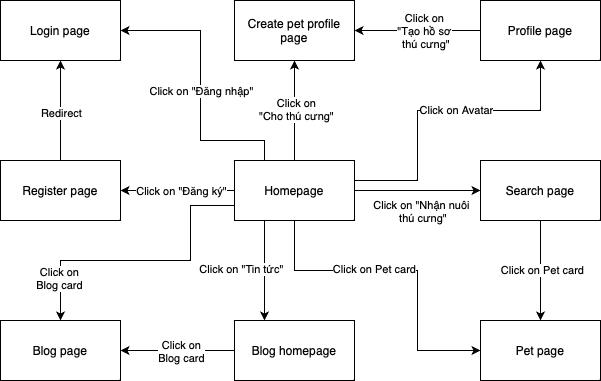
\includegraphics[width=0.8\textwidth]{Figures/wireframe_fo.png}
    \caption{Wireframe for Front office}
\end{figure}

\subsubsection{Homepage}

The homepage serves as the focal point of our pet adoption website, designed with a user-centric approach to ensure an intuitive and engaging experience. The navigation bar stands as a gateway to key functionalities, allowing users to seamlessly register, log in, explore pet profiles, create their pet profiles, access insightful blog content, and manage their user profile. The strategic placement of these navigation options facilitates effortless interaction. The hero section captures attention with visually appealing imagery and succinct messaging, encapsulating the essence of our mission. The "About Us" section provides a deeper understanding of our organization, building trust and connection with our audience. Additionally, the organization section offers insights into our partners and collaborators, fostering a sense of community.

\begin {figure}[H]
\centering
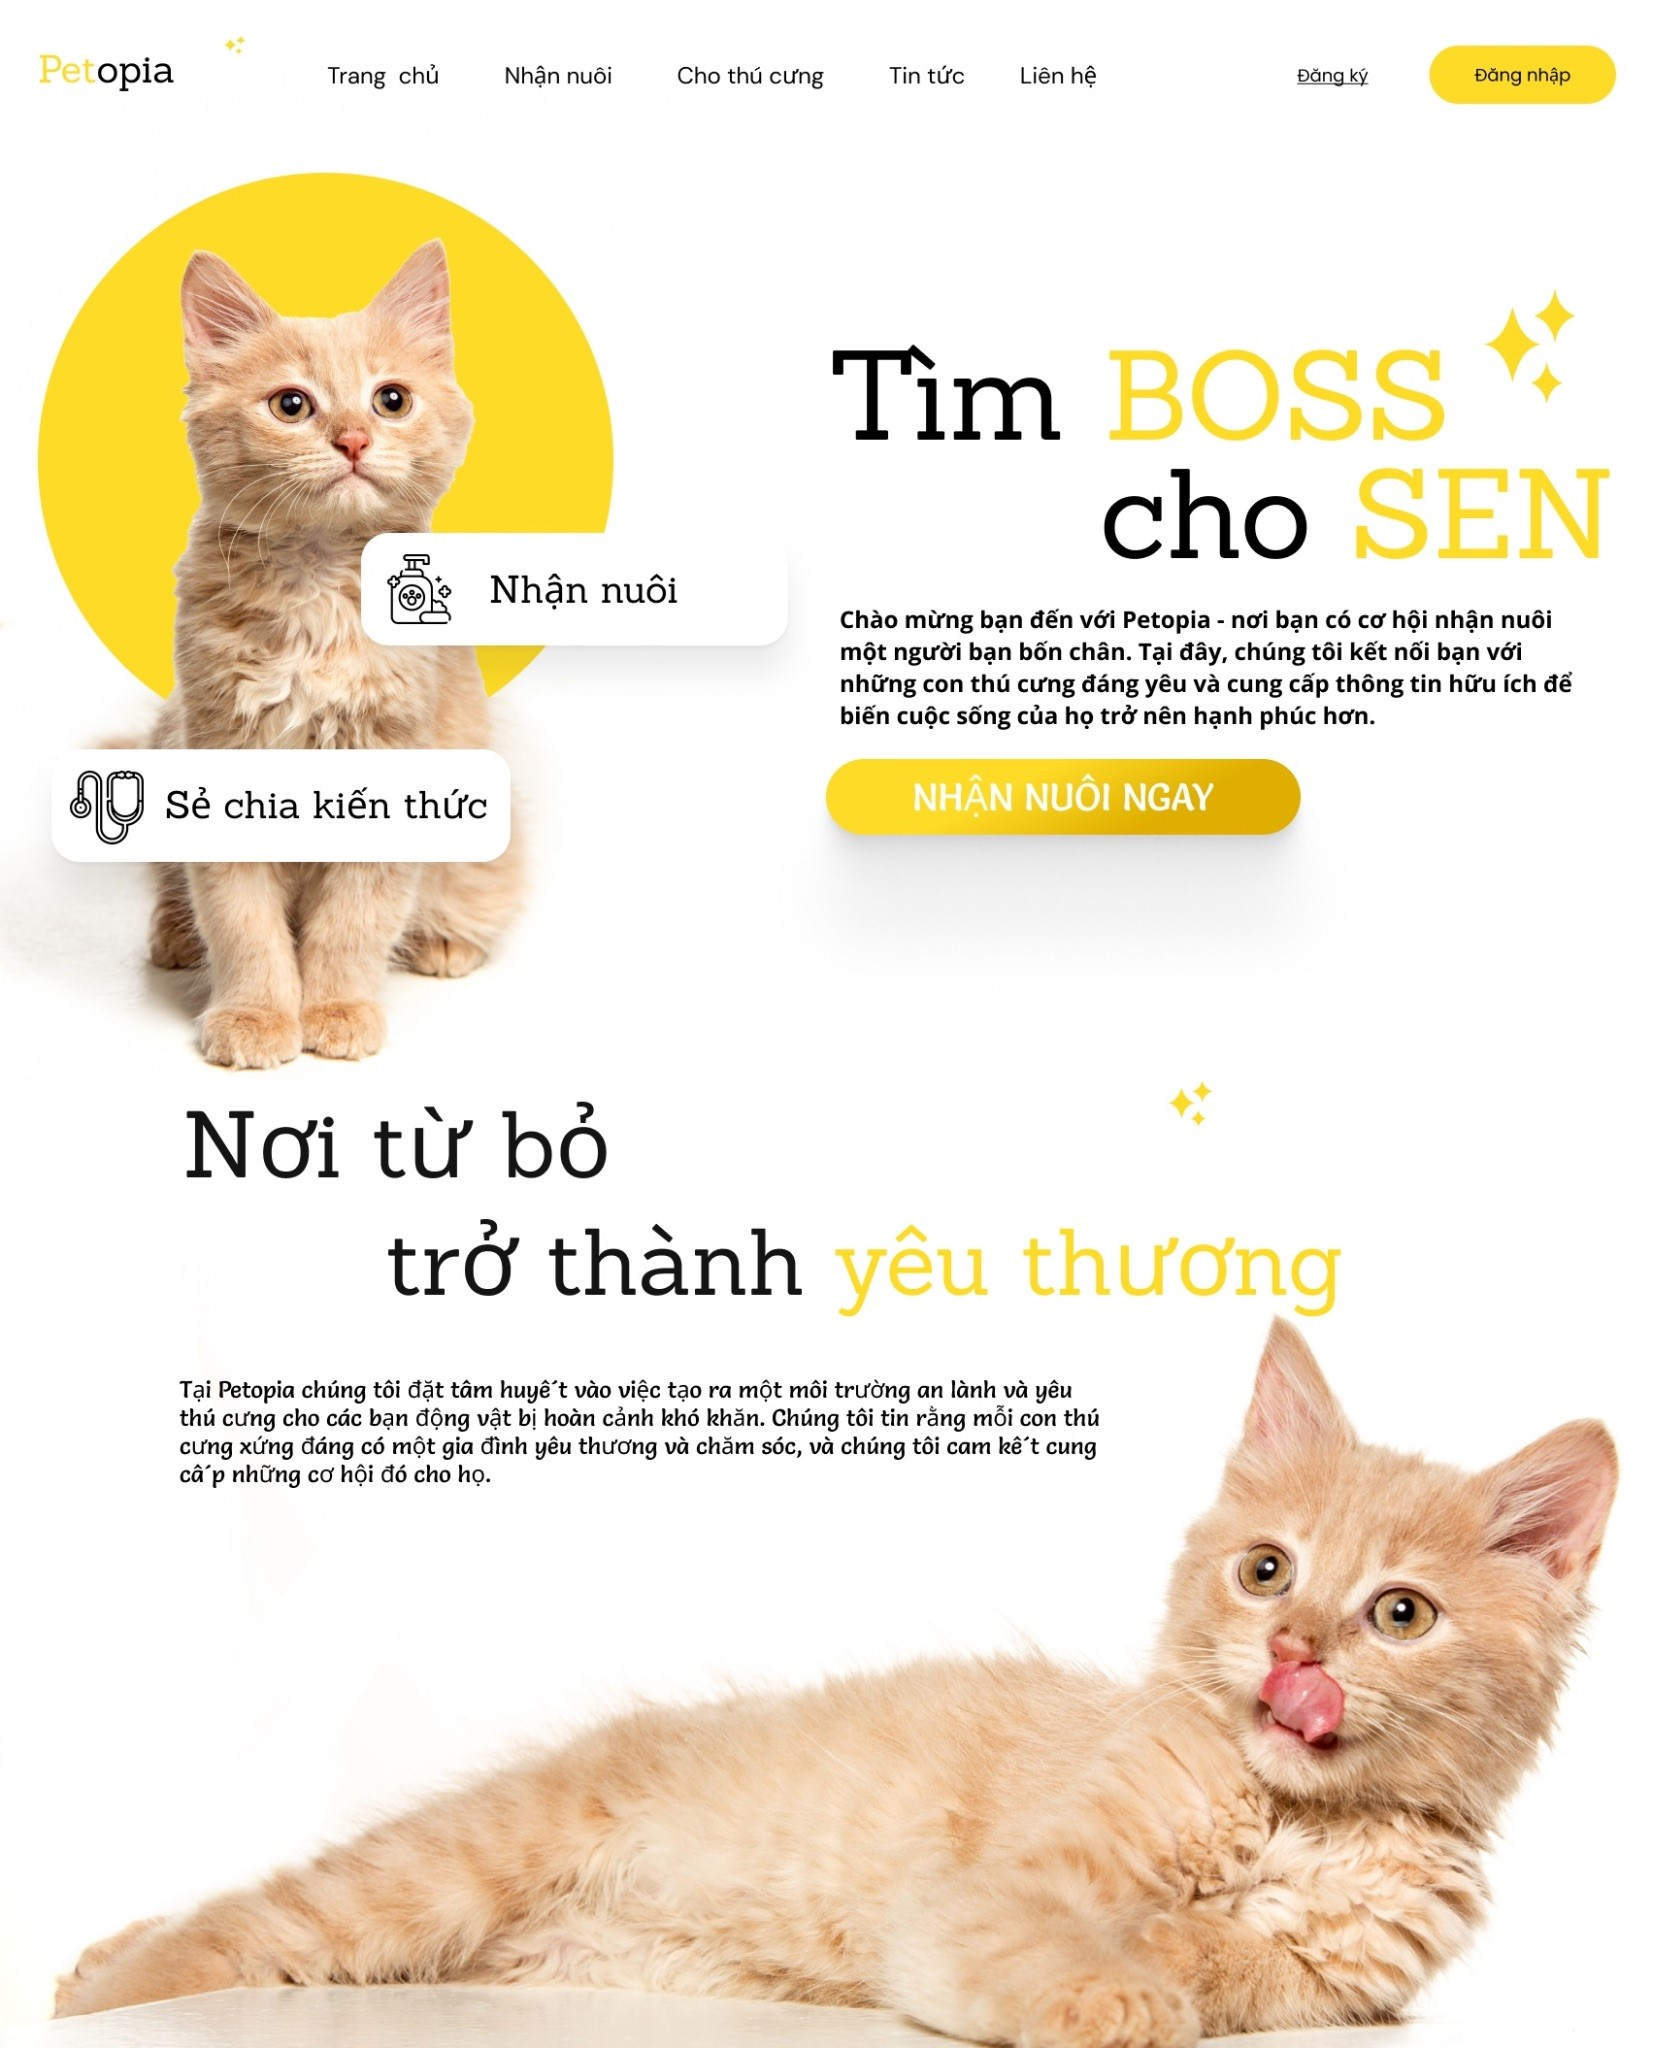
\includegraphics[width=0.8\textwidth]{Figures/UI/home_ui.jpg}
\caption{Homepage of Petopia}
\end{figure}

\subsubsection{Login}

Our homepage's login functionality is designed for simplicity and security, providing a seamless entry into the pet adoption experience. Users can access the login page with a click on the "Đăng nhập" button, where they input their Gmail and password. Error notifications guide users in case of issues, and a convenient register button directs new users to the registration page. For accessibility, users can also log in using their Google account, streamlining the process. A "Forgot Password" option is available for password resets, ensuring a hassle-free and secure experience that accommodates diverse user preferences.

\begin{figure}[H]
    \centering
    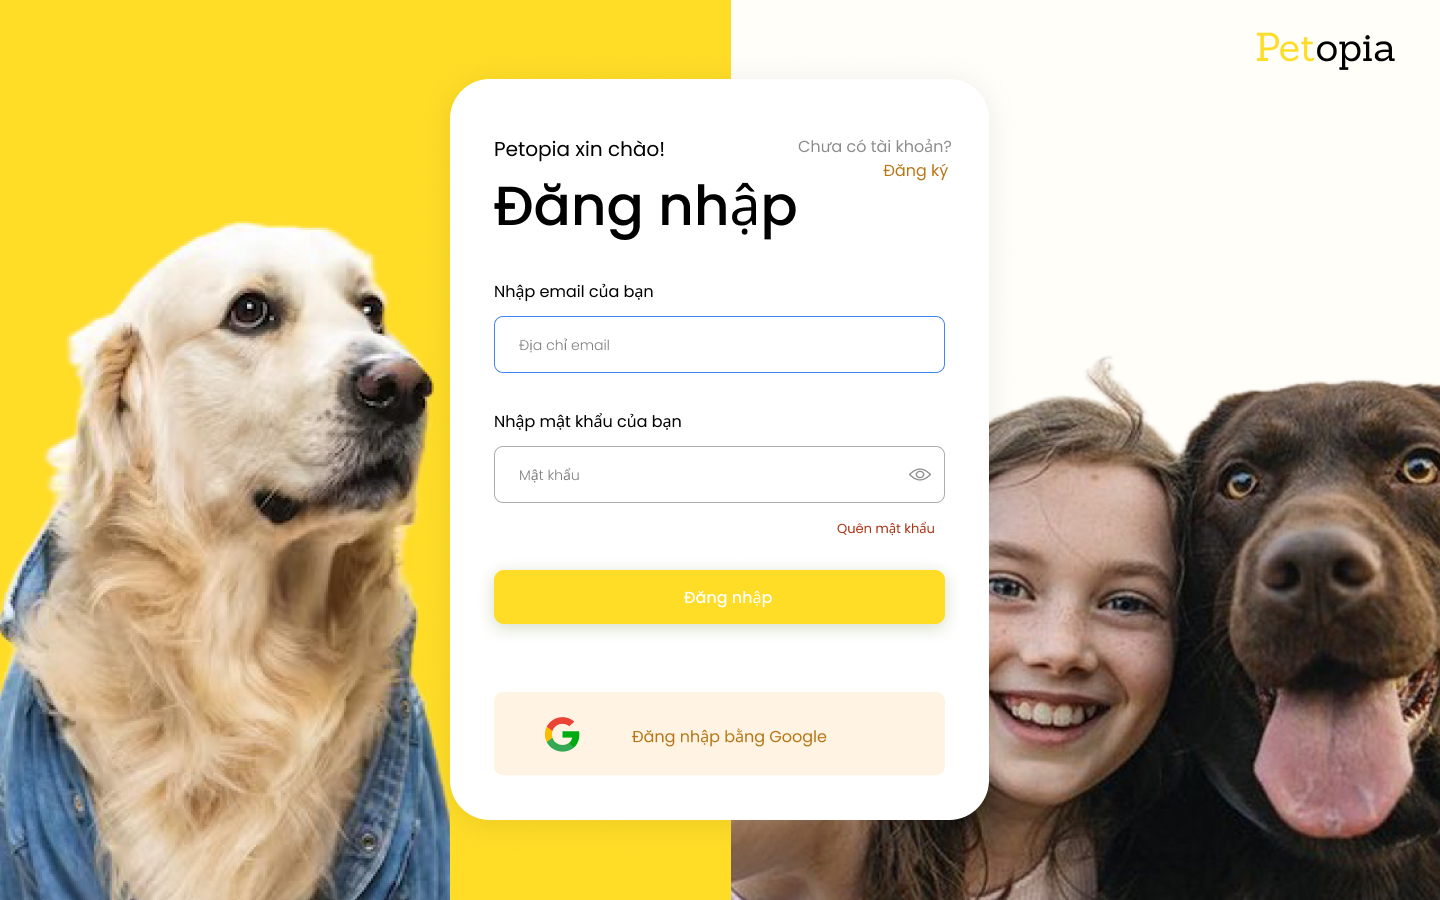
\includegraphics[width=0.8\textwidth]{Figures/UI/login_ui.png}
    \caption{Login form}
\end{figure}

\subsubsection{Register}

The registration process is straightforward, requiring users to input essential information such as first name, last name, Gmail, and password. After clicking "Register," the system verifies the form's completeness and prompts users to check their email for account verification. A verification link enhances security, ensuring authenticity. Clicking the link redirects users to the login page, confirming successful account creation. This two-step process prioritizes security and user-friendly guidance, fostering trust in our platform.

\begin{figure}[H]
    \centering
    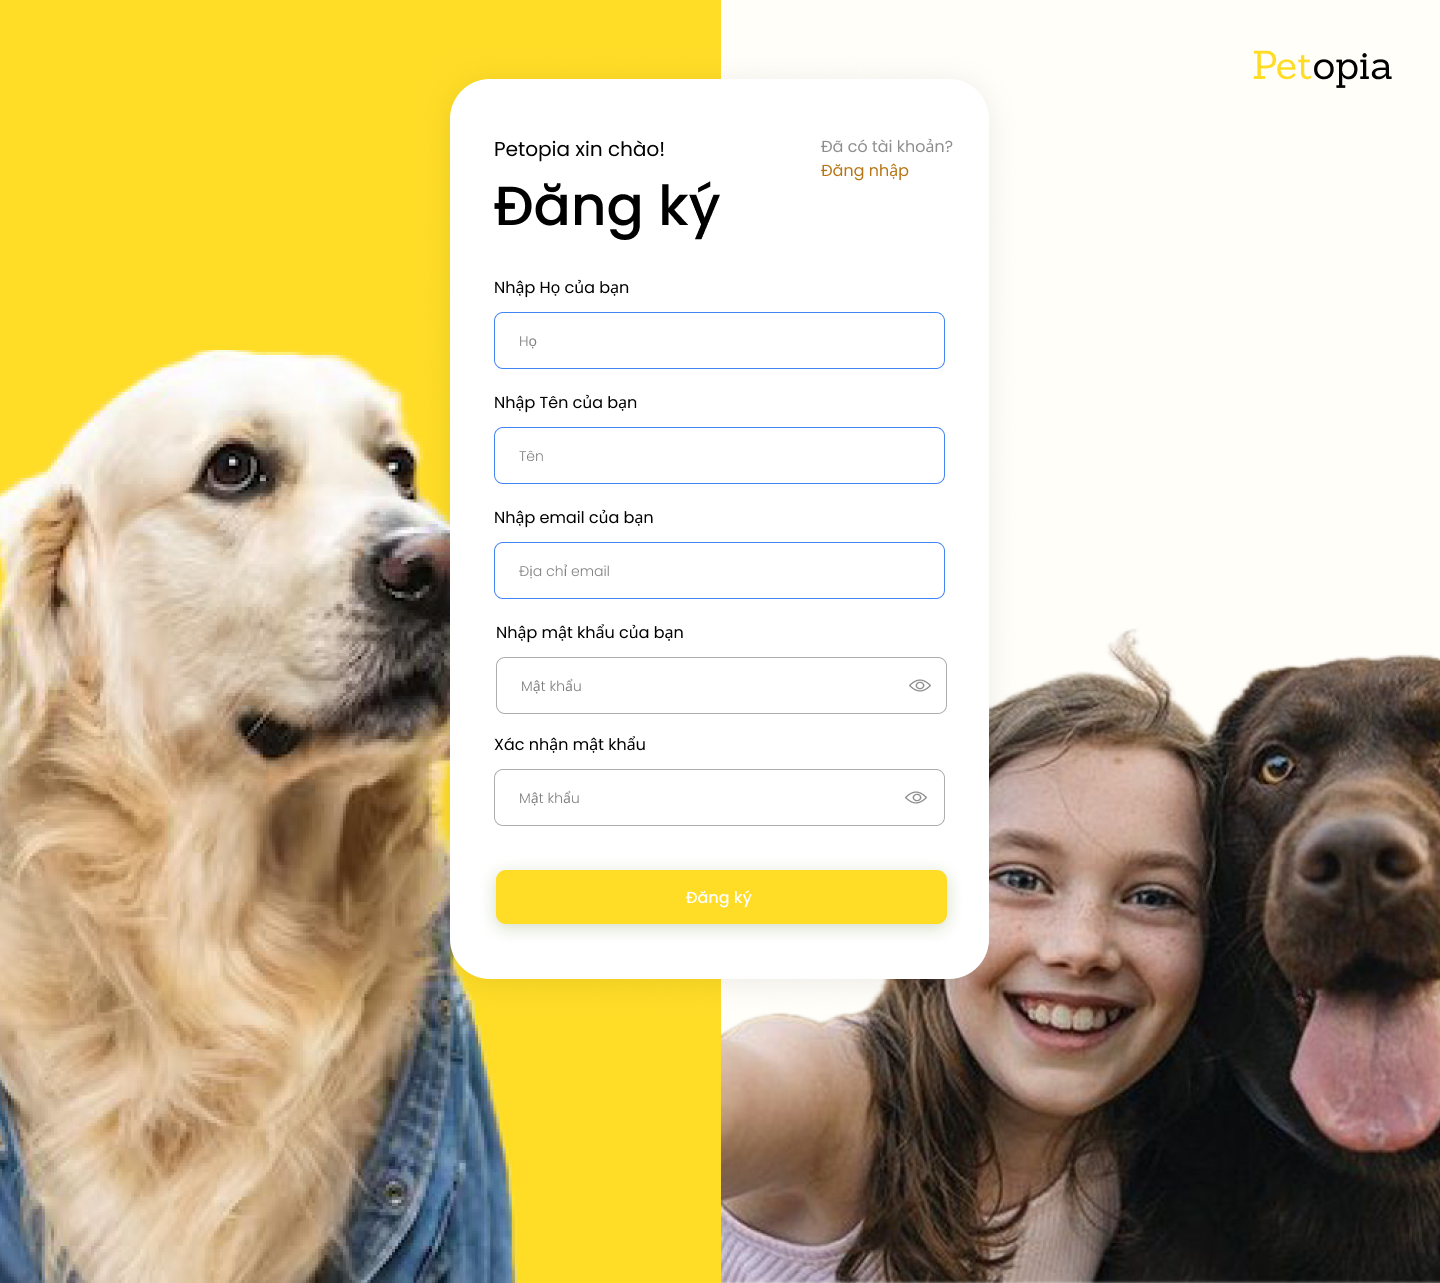
\includegraphics[width=0.5\textwidth]{Figures/UI/register_ui.png}
    \caption{Register form}
\end{figure}

\subsubsection{Search page}

The pet search page is designed for precision and ease. Users can tailor their search 
with checkboxes for sex, breed, color, size, and vaccination status. A sorting feature 
arranges results for flexibility. A prominent search bar, and supporting text and image
 queries, ensure a personalized and efficient experience. Robust filtering, sorting, and 
 versatile search methods aim to provide a user-friendly pet discovery journey on our platform.

\begin{figure}[H]
    \centering
    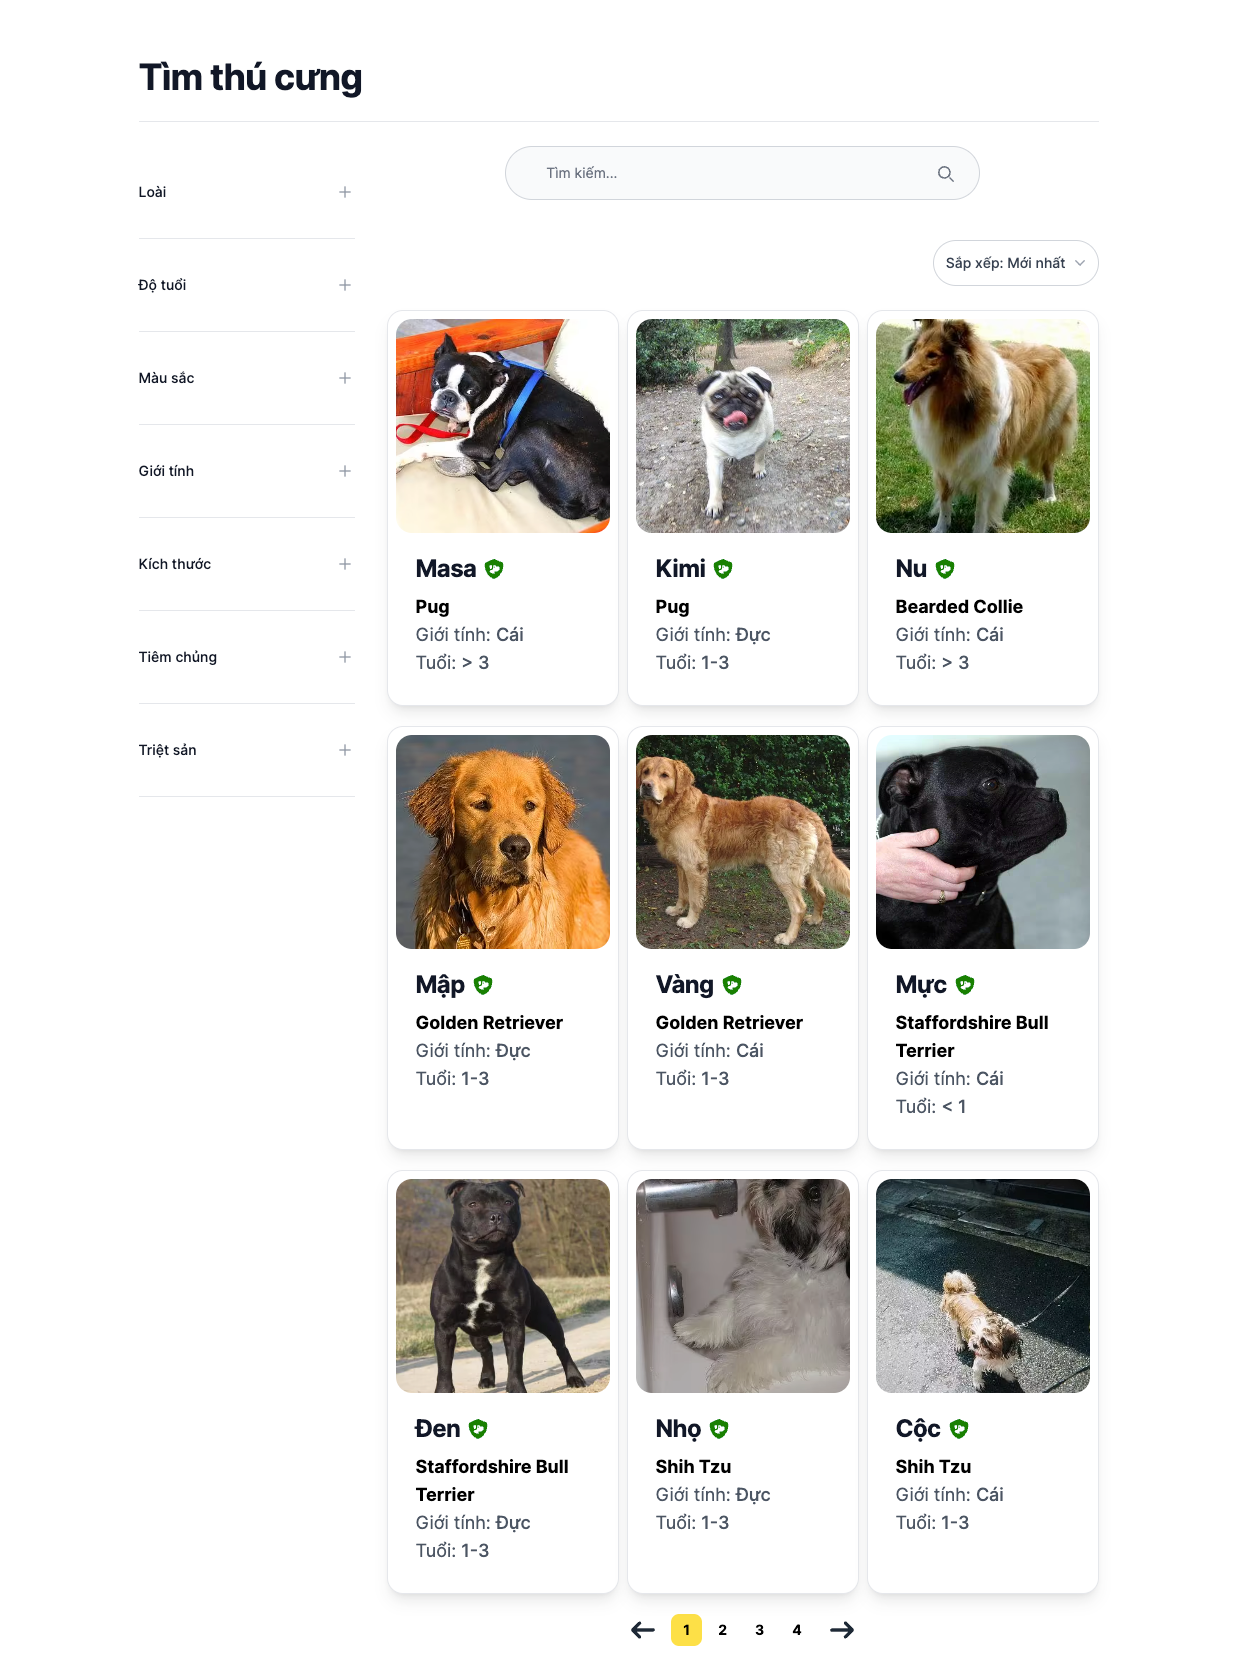
\includegraphics[width=0.8\textwidth]{Figures/UI/search_ui.png}
    \caption{Search page for searching desired pet}
\end{figure}


\subsubsection{Pet profile}

The pet page is a comprehensive showcase, providing detailed insights into each pet. Clicking on a pet card redirects users to the dedicated pet profile page, displaying key information such as name, breed, age, and vaccination status. Striking images and a personal description offer a deeper understanding of the pet's personality. A prominent "Adopt" button facilitates the adoption process, dynamically revealing an efficient adoption form upon click. This ensures transparent communication between potential adopters and pet owners.

\begin{figure}[H]
    \centering
    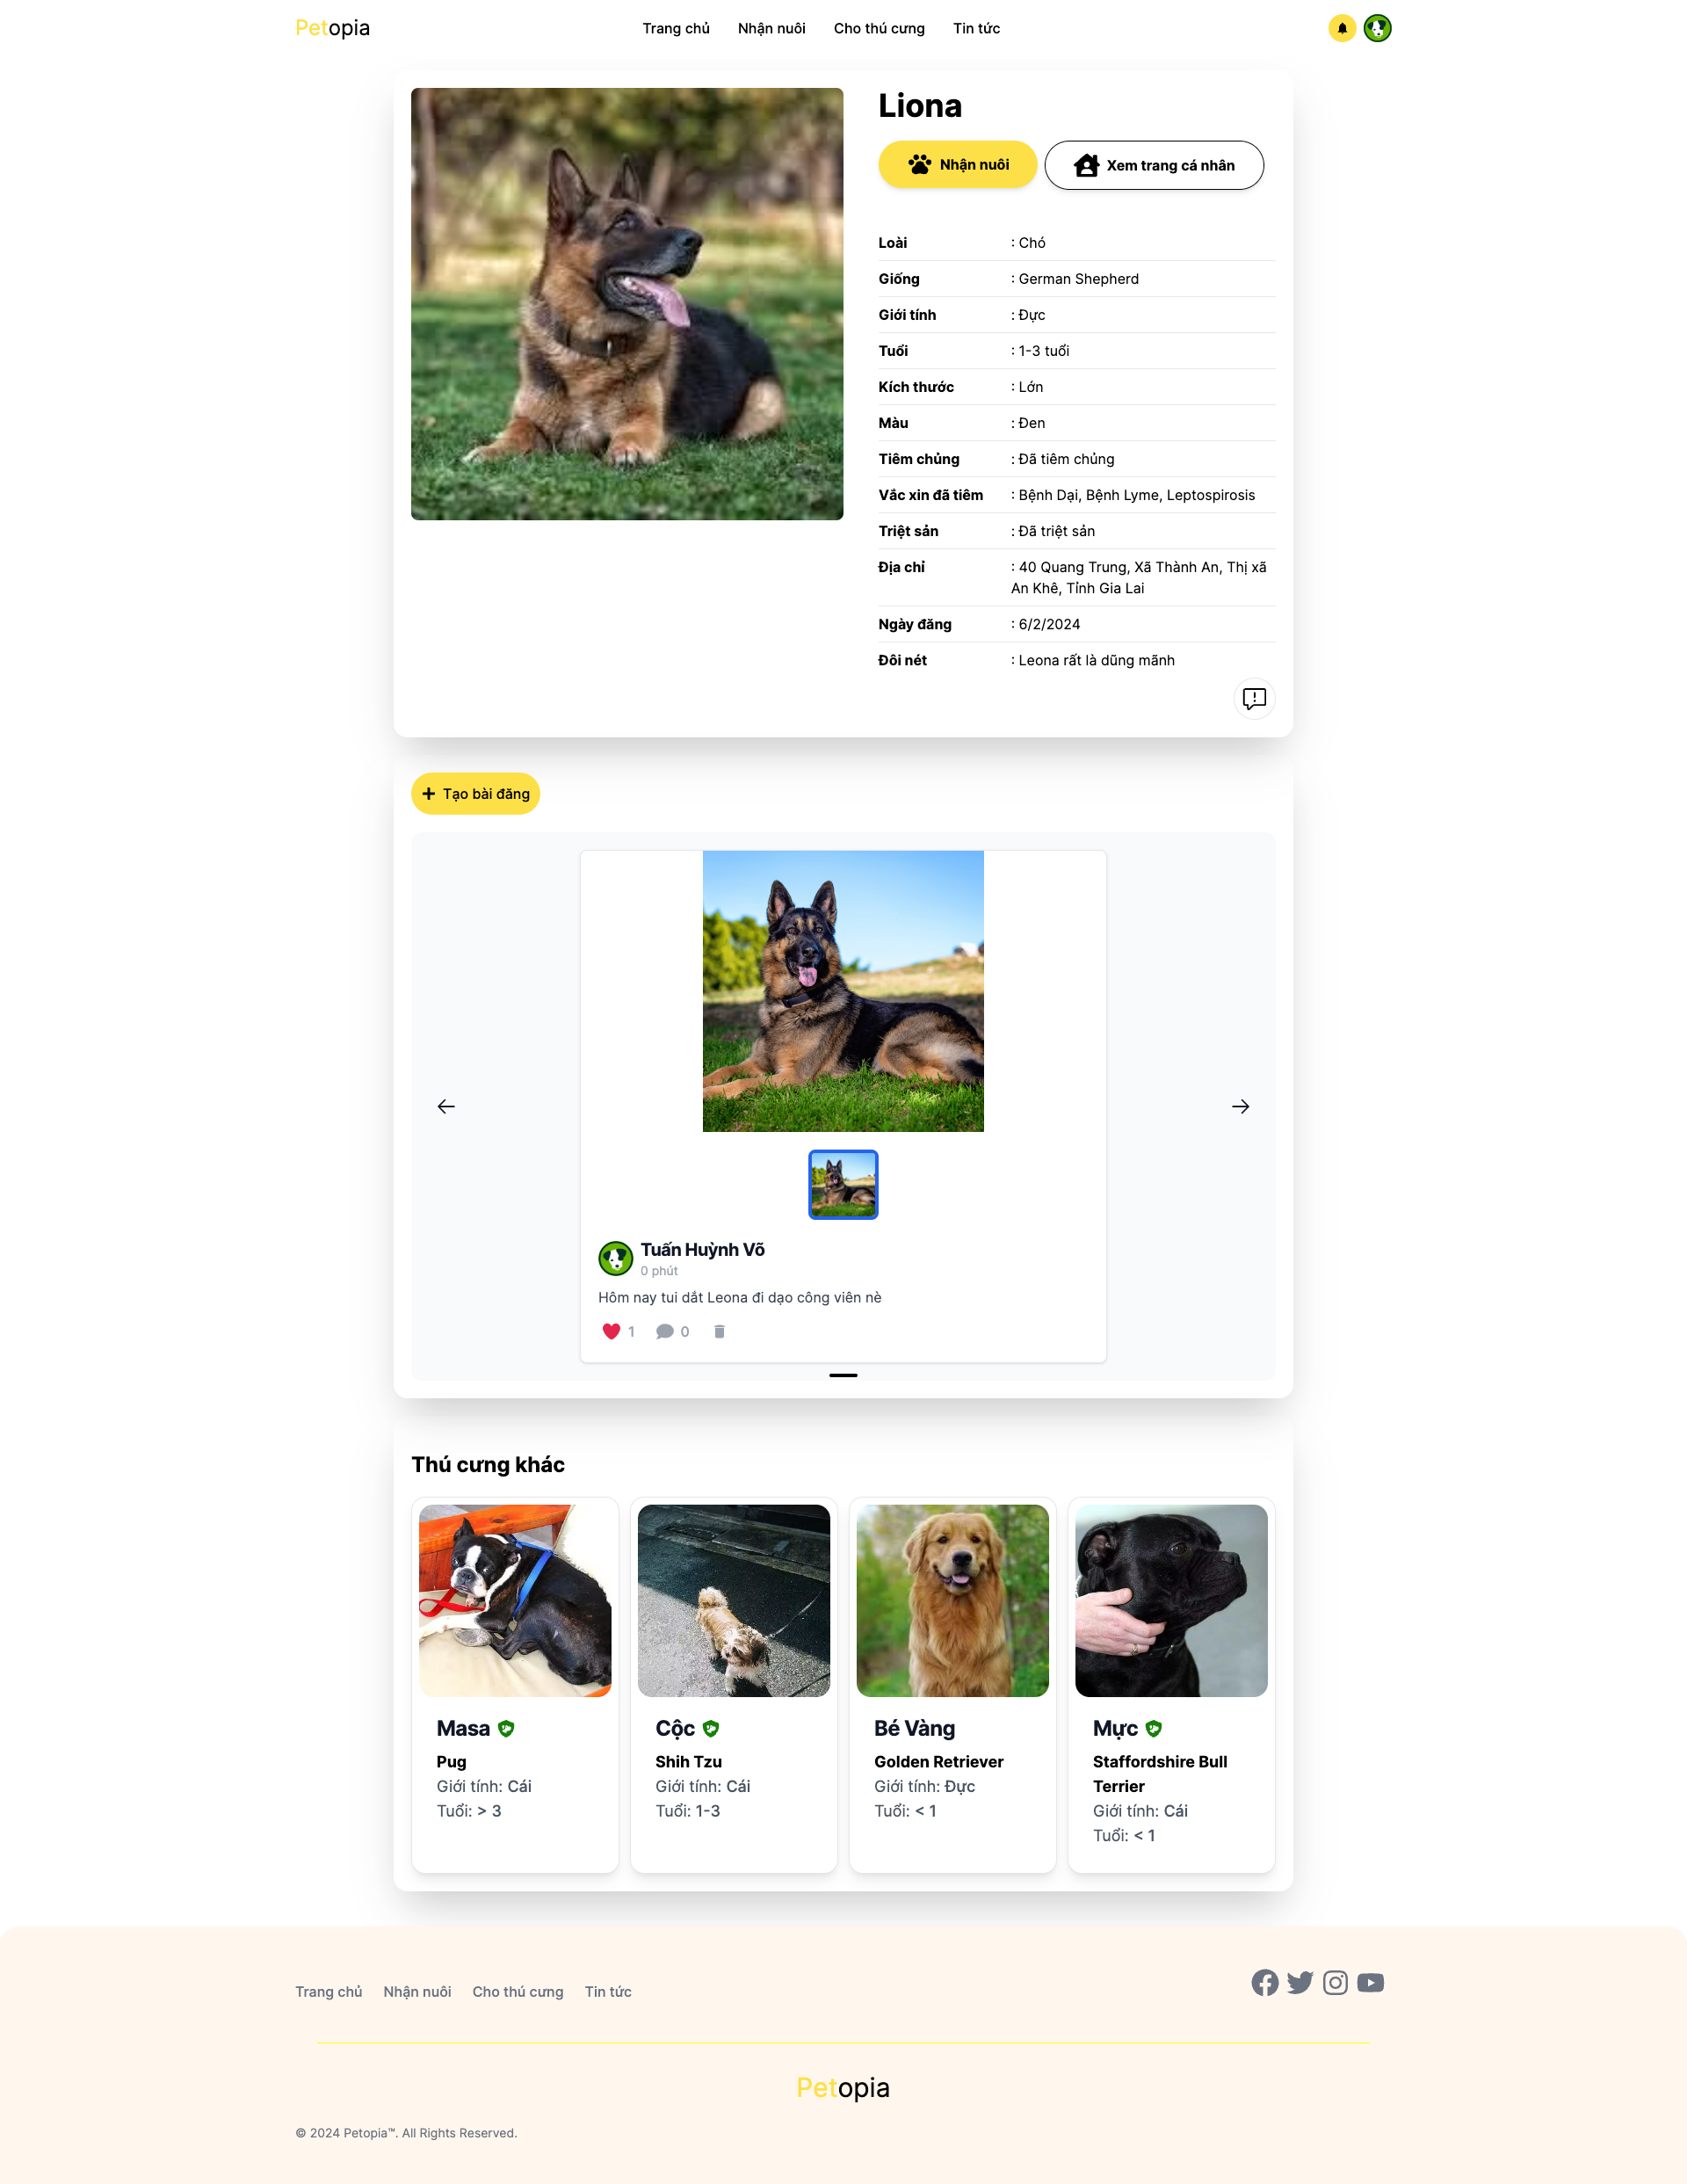
\includegraphics[width=0.6\textwidth]{Figures/UI/pet_detail_ui.png}
    \caption{Pet profile page}
\end{figure}

\subsubsection{Create pet profile}

\begin{figure}[H]
    \centering
    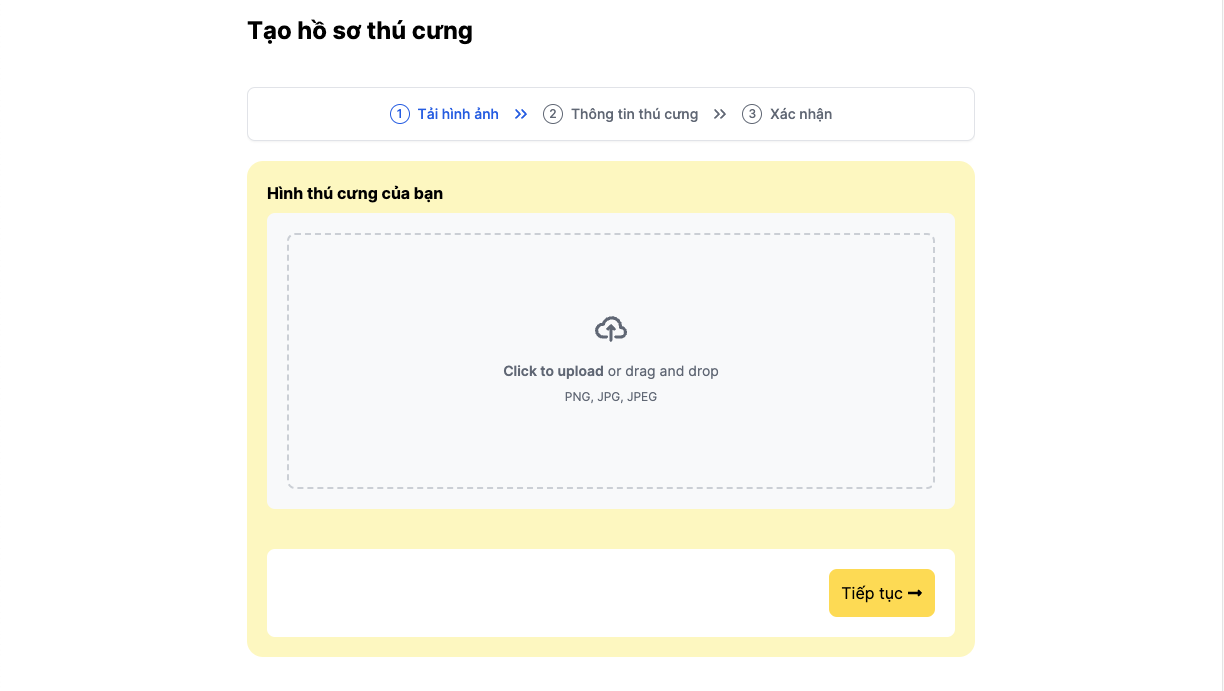
\includegraphics[width=0.6\textwidth]{Figures/UI/image_upload_ui.png}
    \caption{Image upload form}
\end{figure}

\begin{figure}[H]
    \centering
    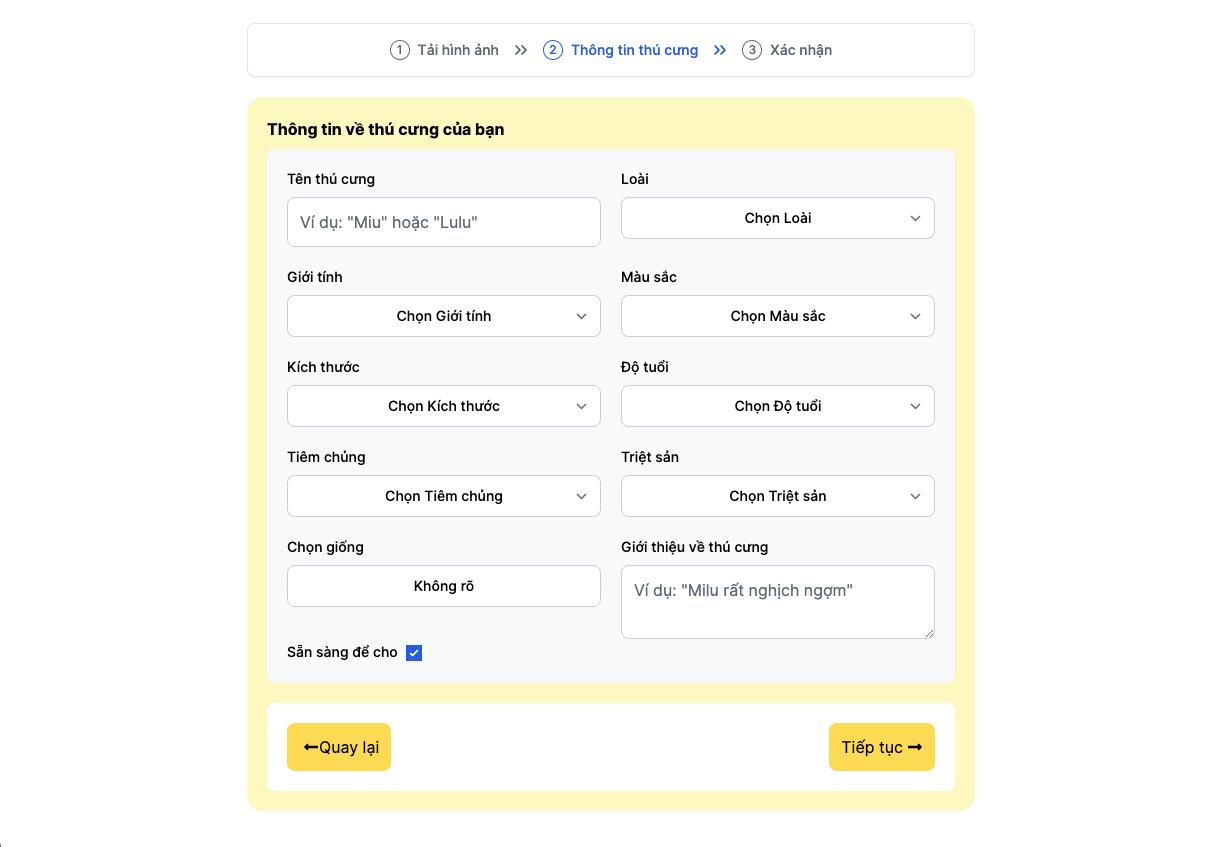
\includegraphics[width=0.6\textwidth]{Figures/UI/pet_input_ui.png}
    \caption{Form for taking user's pet detail}
\end{figure}

\begin {figure}[H]
\centering
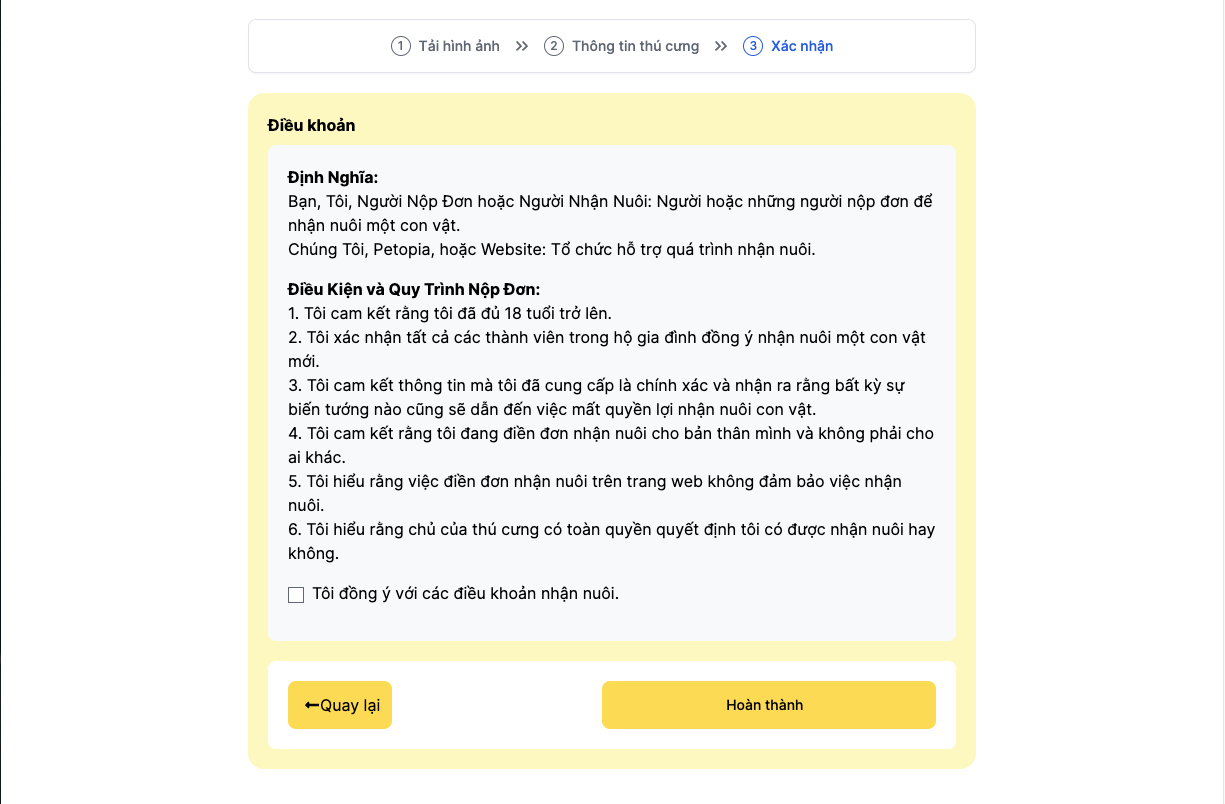
\includegraphics[width=0.6\textwidth]{Figures/UI/term_ui.png}
\caption{Pet profile page}
\end{figure}

Creating a pet profile on our platform is user-friendly and efficient. Users begin by uploading a pet image (Figure 3.8), which our AI processes to autofill the breed. Clicking "Continue" leads to a detailed pet form (Figure 3.9) for additional information. Users then review the Terms and Services (Figure 3.10) before clicking "Finish" to complete the profile. This structured process, with AI assistance in the initial steps, ensures accuracy and a seamless user experience.

\subsubsection{User profile}

\begin{figure}[H]
    \centering
    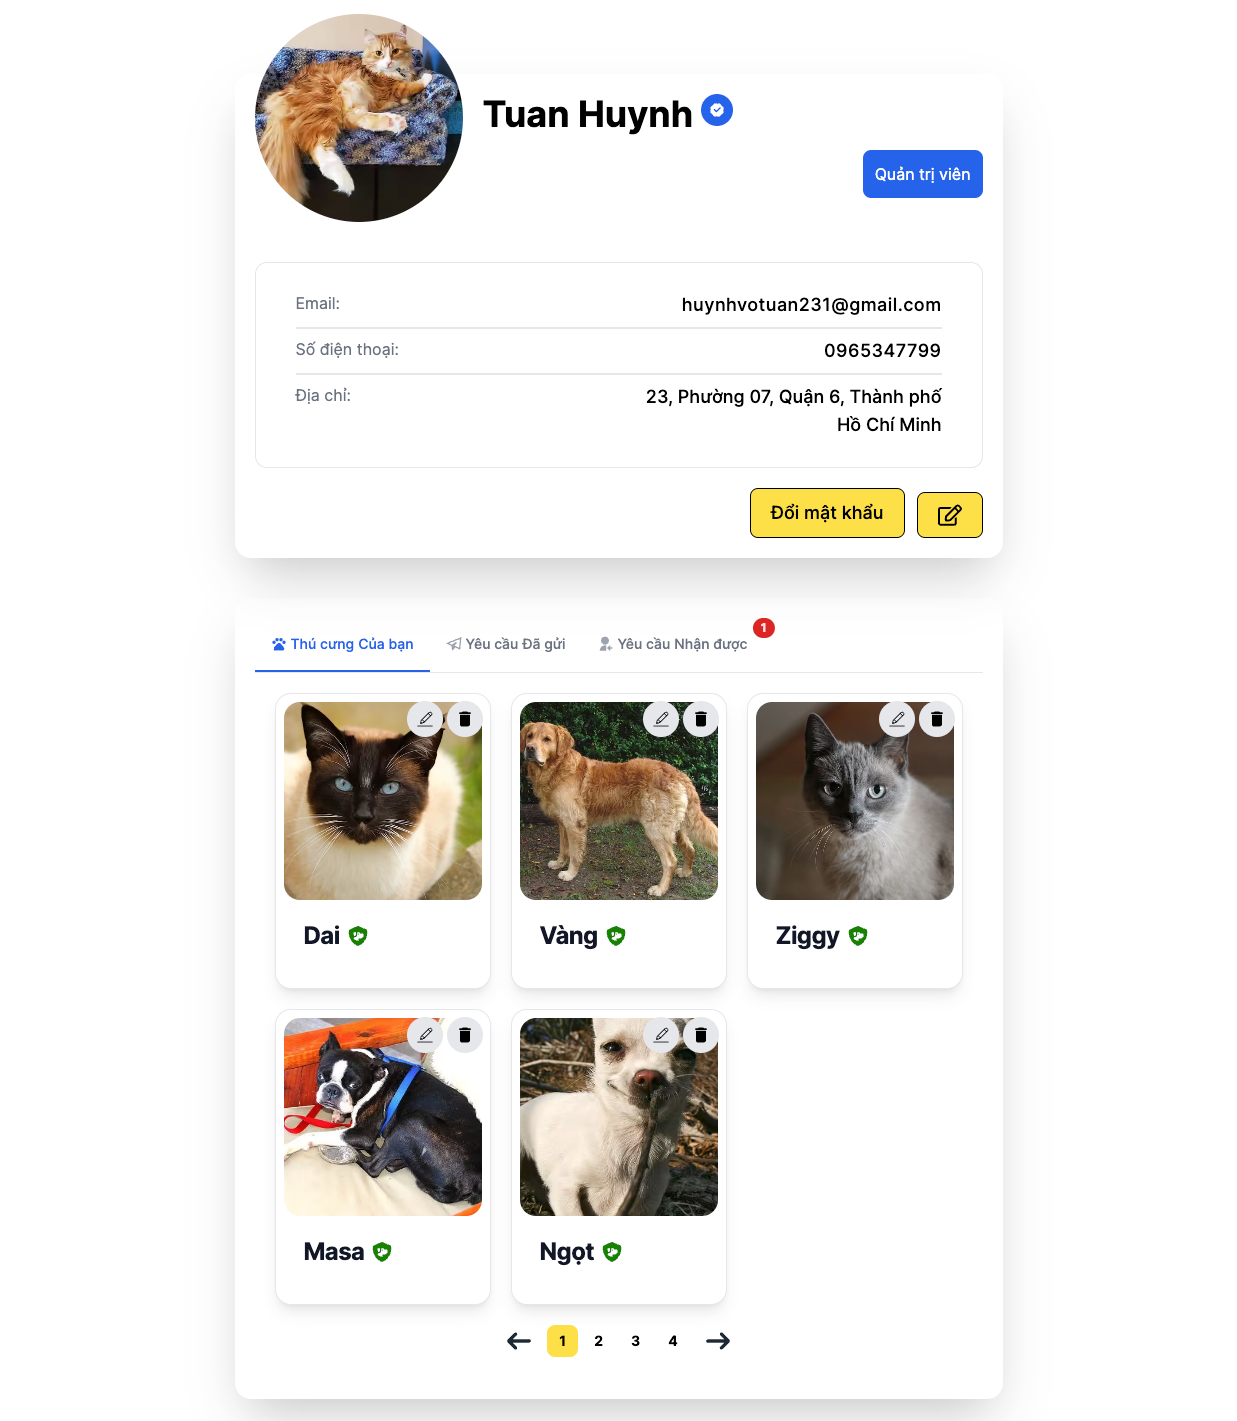
\includegraphics[width=0.7\textwidth]{Figures/UI/user_profile_ui.png}
    \caption{User profile page}
\end{figure}
The user profile page serves as a centralized hub for managing and personalizing 
information, offering a seamless and enjoyable experience. At the top, users will 
find their avatar, name, address, Gmail, and phone number, all of which can be easily 
edited to keep details up-to-date. User can also change their password or update information in this page. The page also features pet profiles, allowing 
users to manage information about their pets effortlessly. Additionally, a management
 table includes tabs for Sent and Incoming messages, notifying users about adoption
  requests and the status of their adoption forms. This intuitive design ensures 
  users can efficiently handle personal information and engage with our platform's
   pet adoption features.

\subsubsection{Organization profile}
\begin{figure}[H]
    \centering
    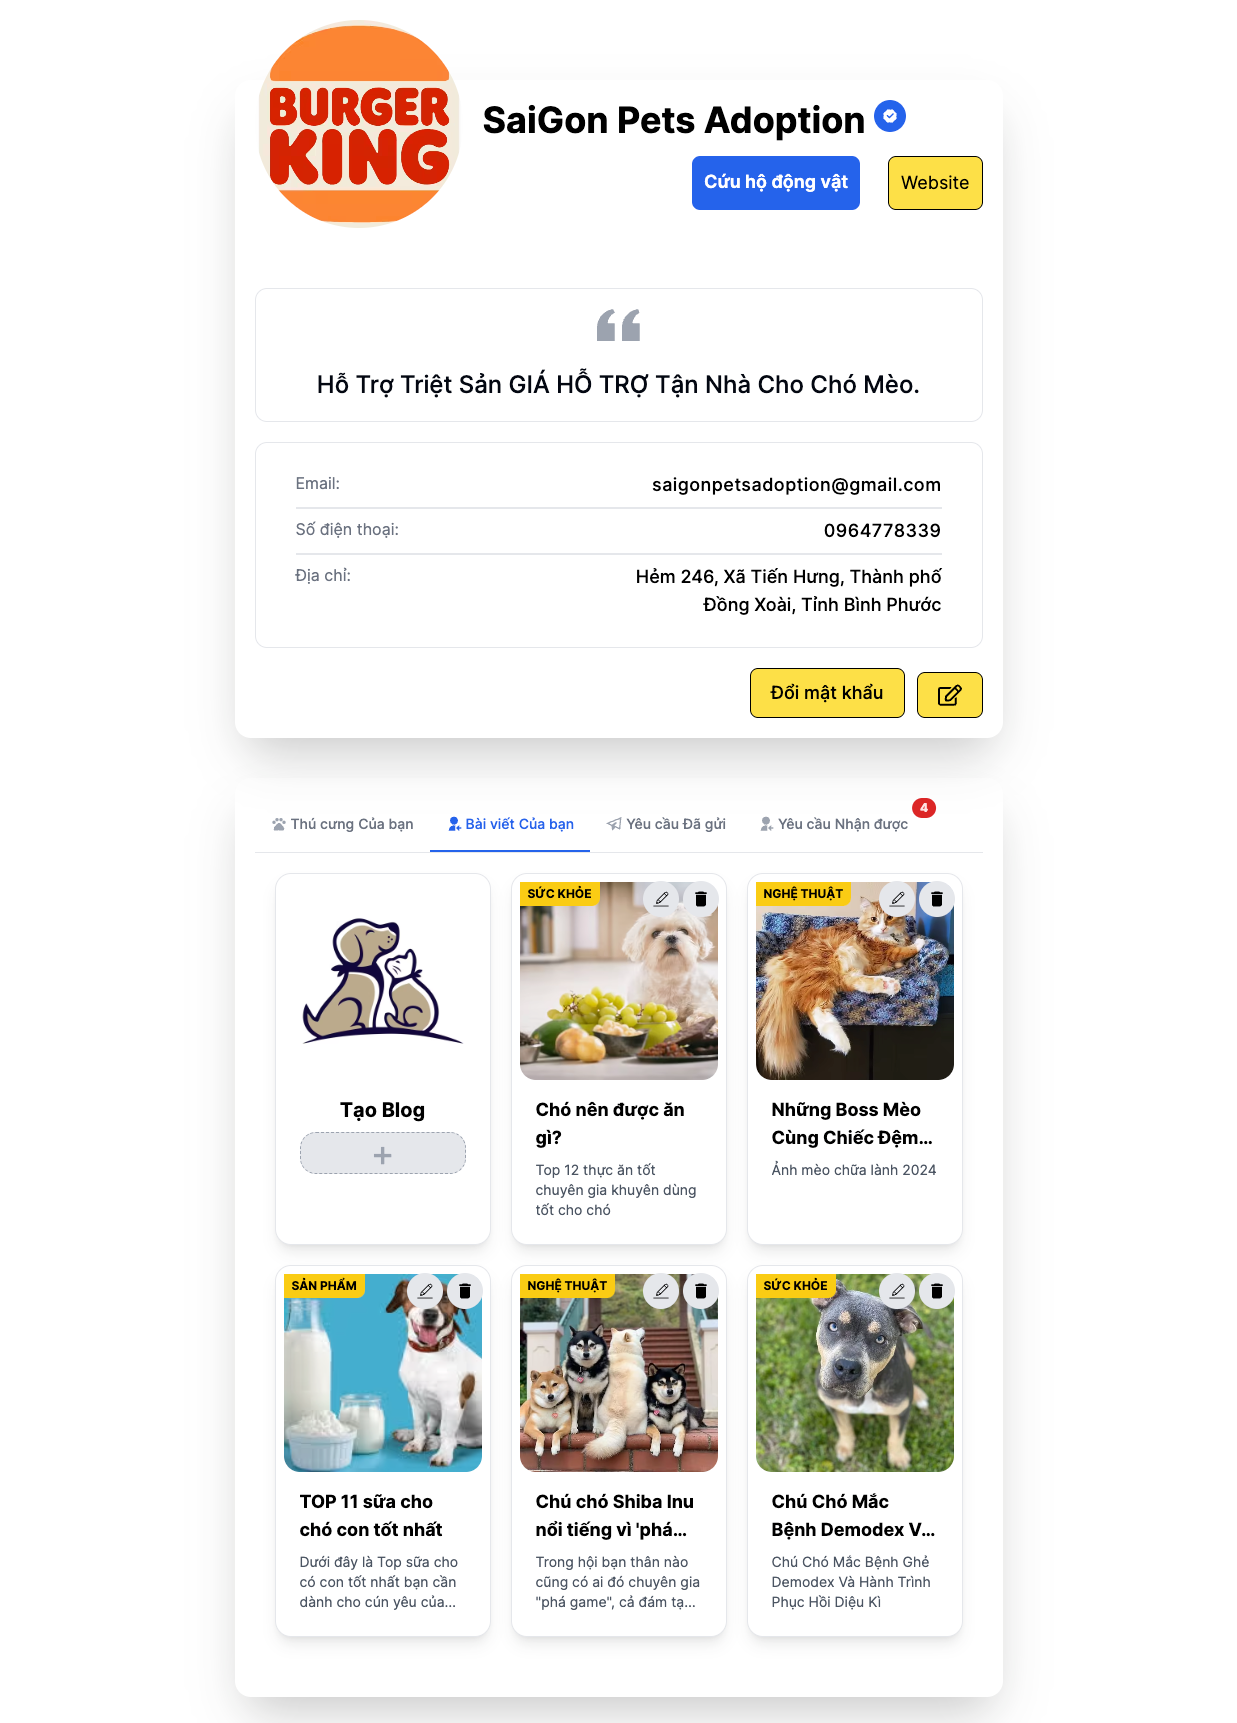
\includegraphics[width=0.7\textwidth]{Figures/UI/org_profile_ui.png}
    \caption{Organization profile page}
\end{figure}

The organization profile mirrors the user profile but includes a verification badge to confirm the account's authenticity. Beneath the organization name, a badge indicates the type of organization. This page also offers functions for changing passwords and updating information. In addition to basic details, the page includes the organization's slogan and web link. The management table features an extra blog tab, allowing users to create, update, or delete blog posts.

\subsubsection{Blog homepage}
\begin{figure}[H]
    \centering
    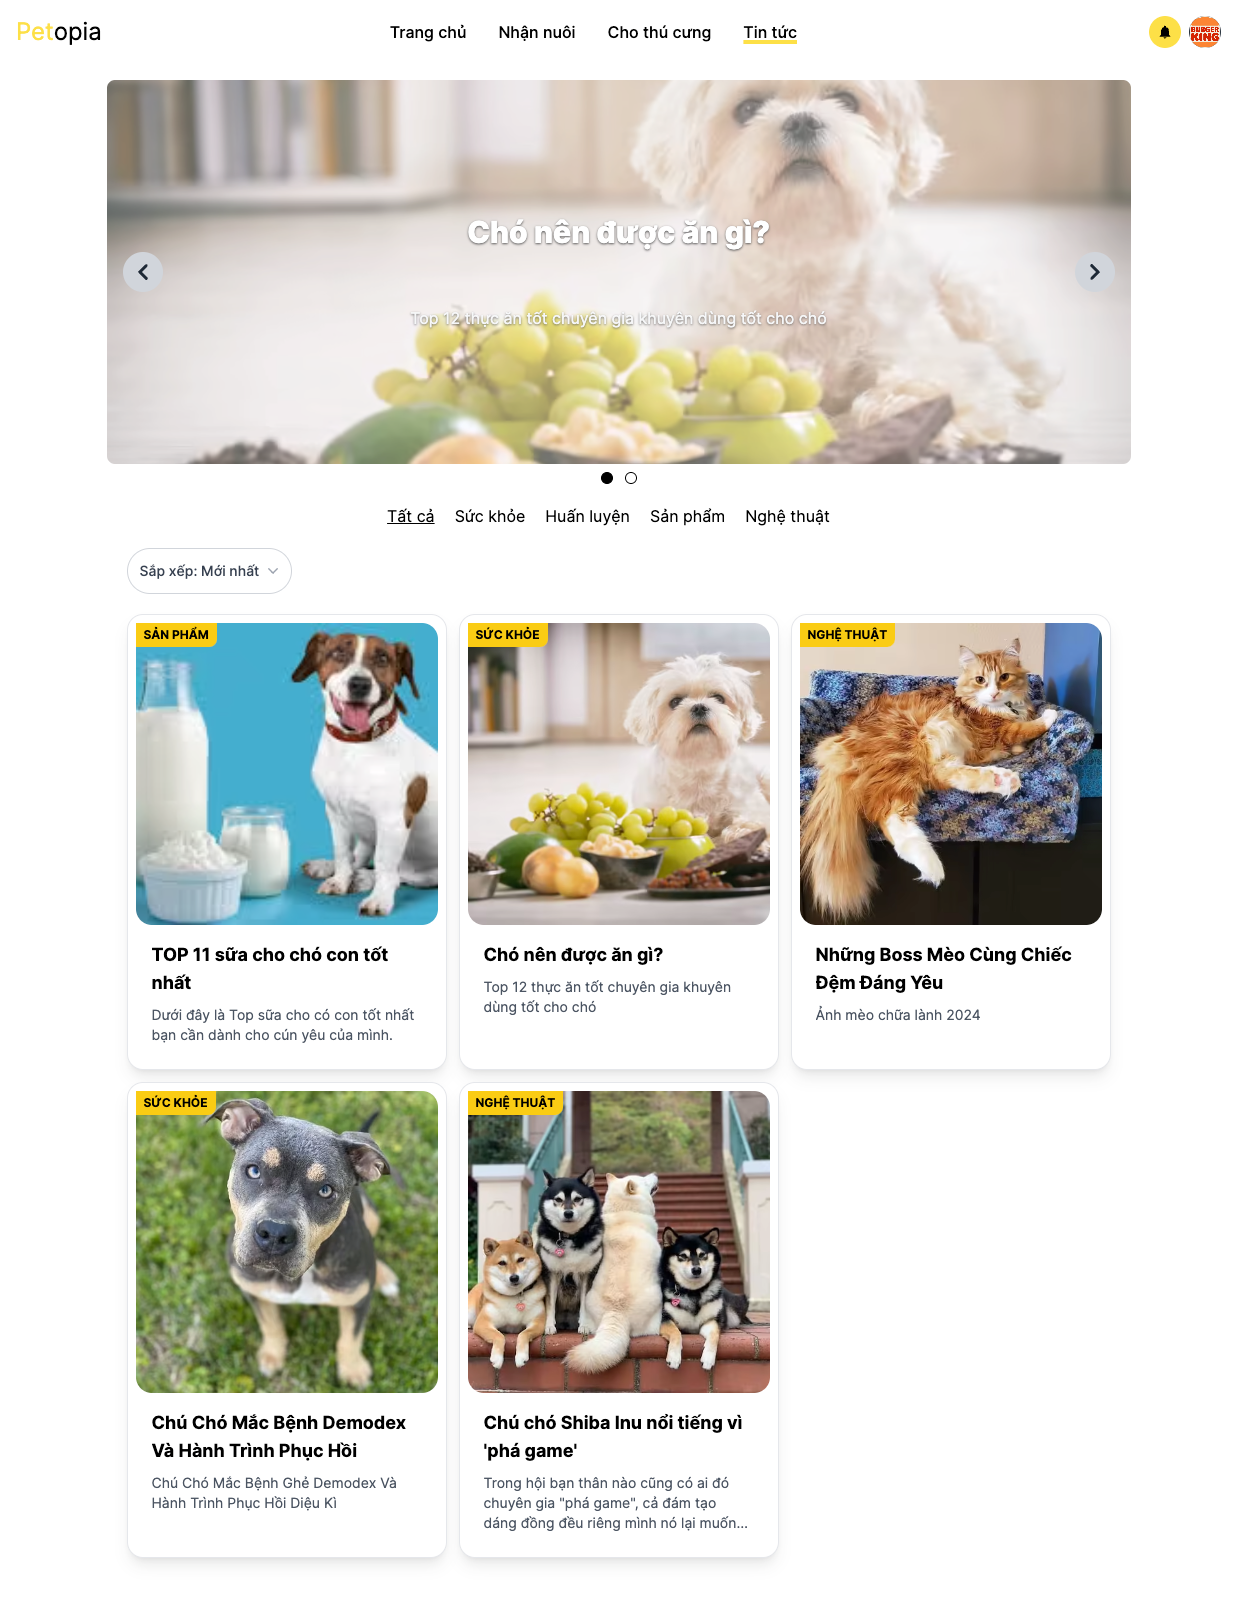
\includegraphics[width=0.8\textwidth]{Figures/UI/blog_ui.png}
    \caption{Blog homepage}
\end{figure}

The blog homepage offers a curated space with various categories for users to explore diverse content.
 Clicking a category dynamically displays relevant blogs, ensuring a targeted reading experience. 
 Selecting a specific blog seamlessly redirects users to the dedicated blog page for detailed 
 exploration. Integrated ads support the platform without disrupting the user experience, 
 contributing to the sustainability of our blog platform.

\subsubsection{Blog page}

\begin{figure}[H]
    \centering
    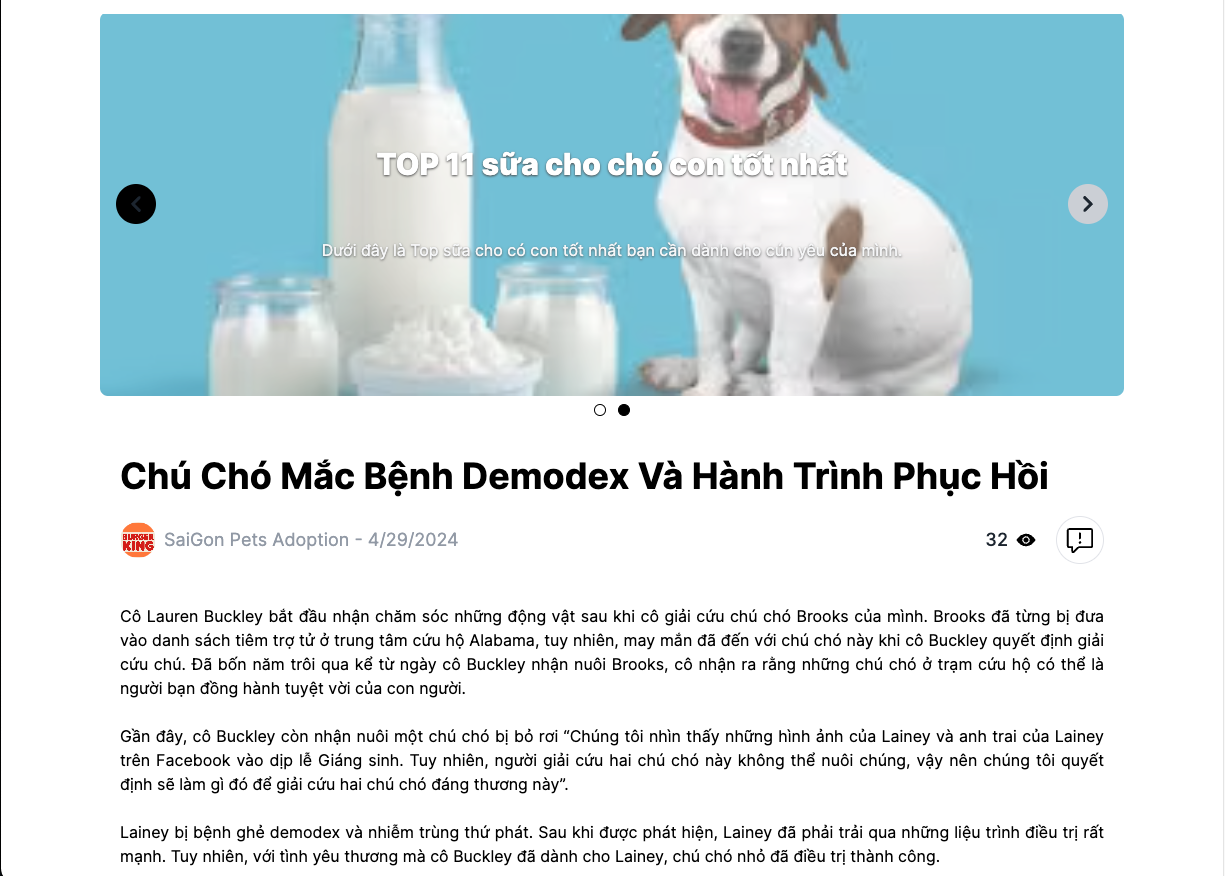
\includegraphics[width=0.8\textwidth]{Figures/UI/blog_page_ui.png}
    \caption{Blog page}
\end{figure}

The blog page ensures a rich and interactive reading experience, allowing users to delve into 
detailed blog posts. Metrics like view count indicate popularity. A relevant section suggests 
related blogs, encouraging users to explore aligned topics for an enhanced and curated experience.

\subsubsection{Payment page}
\begin{figure}[H]
    \centering
    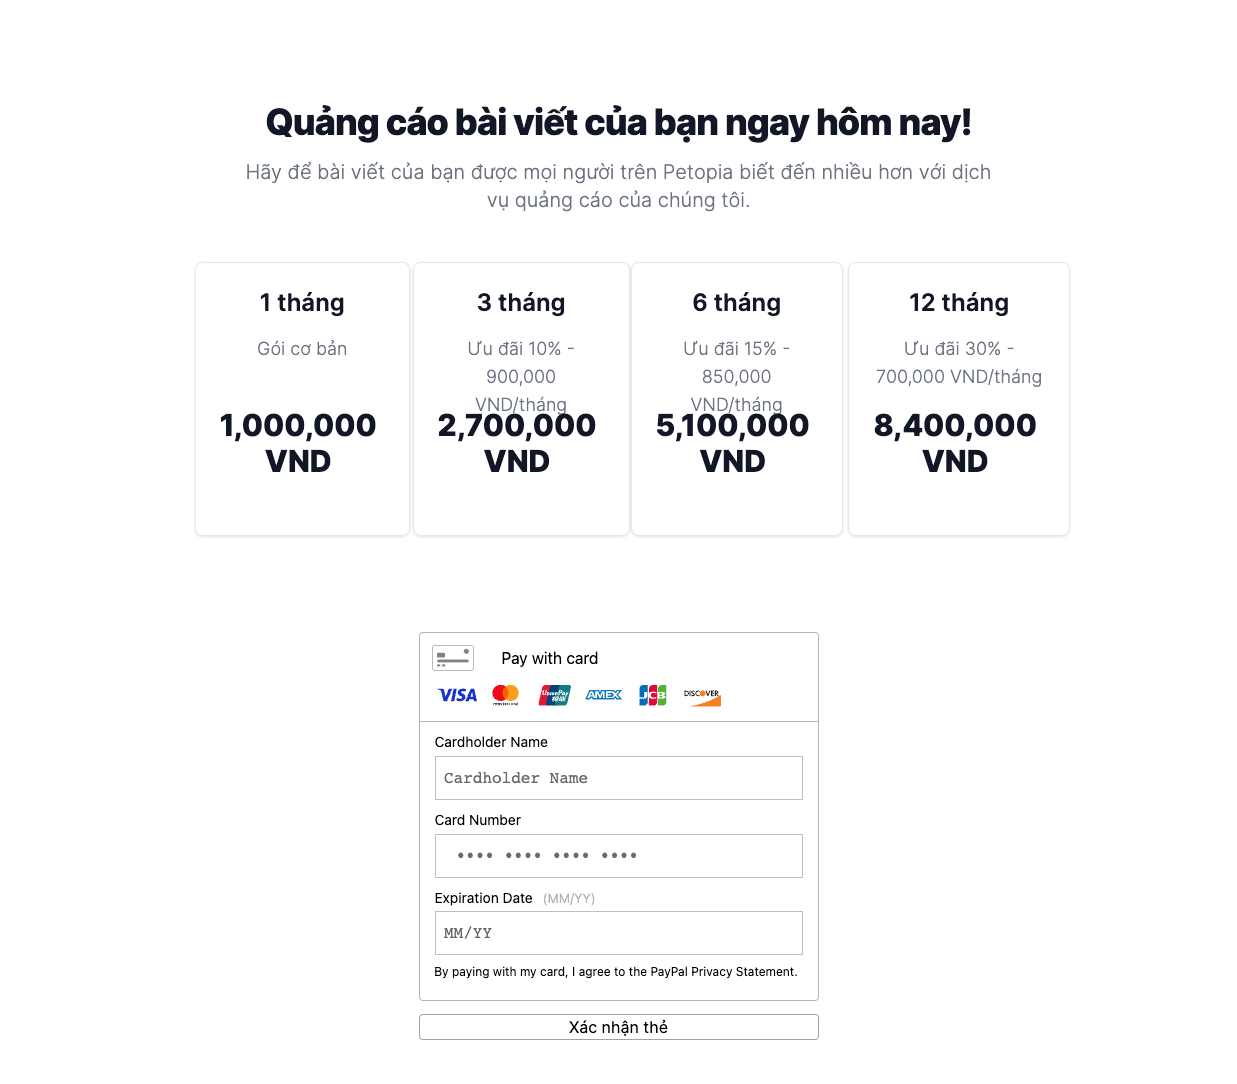
\includegraphics[width=0.8\textwidth]{Figures/UI/payment_ui.png}
    \caption{Payment page}
\end{figure}
On the payment page, users have the option to advertise their blog by selecting from one of four subscription plans: 1 month, 3 months, 6 months, or 12 months. Each plan offers varying levels of exposure and cost, allowing users to choose the duration that best fits their needs and budget. Once a plan is selected, users can proceed by entering their card information in the provided fields. The system ensures secure processing of the payment, after which the advertising plan will be activated. This streamlined process makes it easy for users to promote their blogs effectively.

\newpage
\subsection{Back office}

\subsubsection{Dashboard}

\begin{figure}[H]
    \centering
    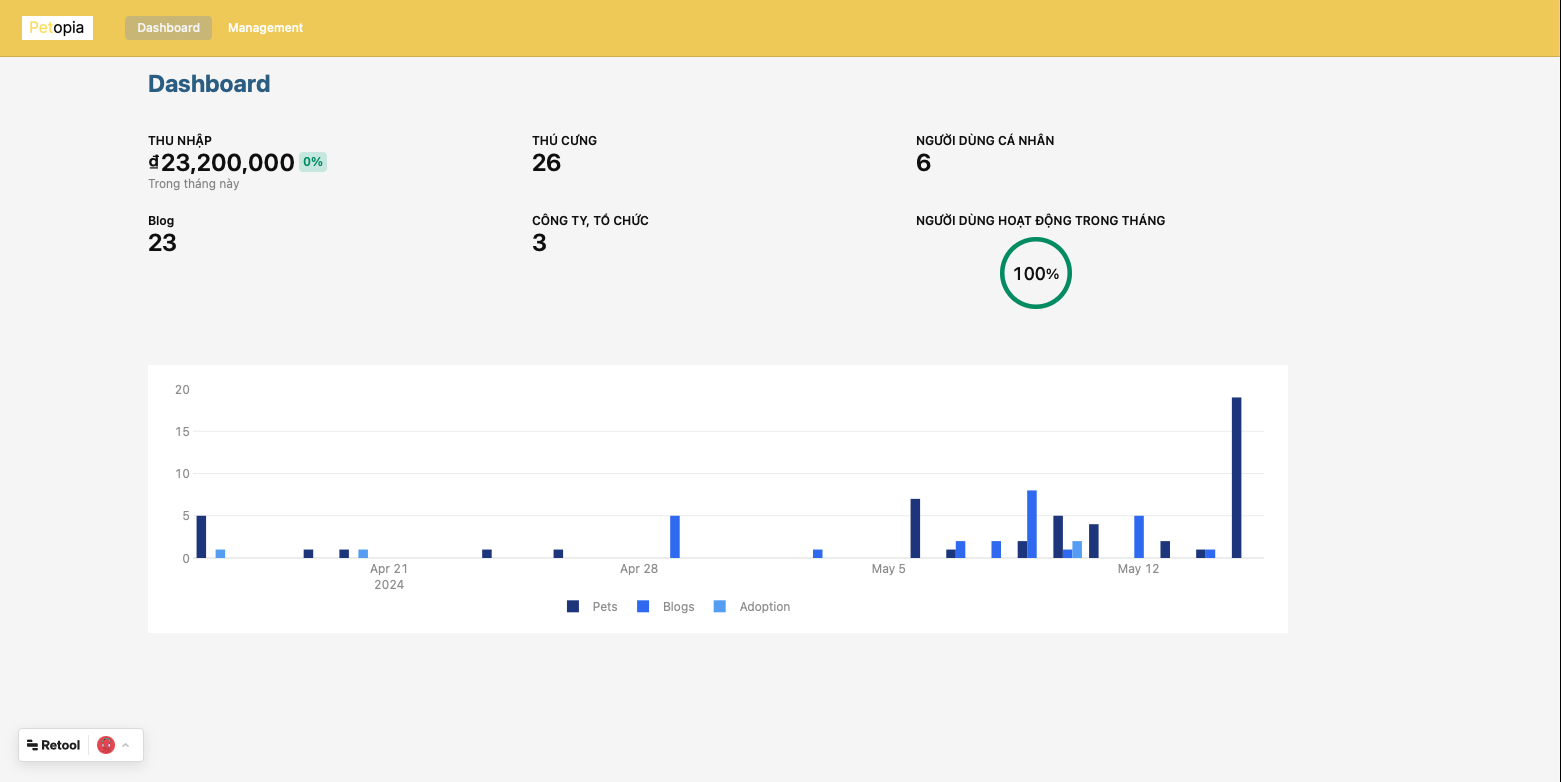
\includegraphics[width=0.7\textwidth]{Figures/UI/dashboard_bo_ui.png}
    \caption{Dashboard to show reports and statistics}
\end{figure}

The dashboard page provides administrators with comprehensive insights into the Petopia website. It displays key metrics such as the number of visitors, pets, blogs, and users. To enhance visualization, graphical representations accompany these statistics, offering a clear and dynamic overview of the platform's performance. This feature allows administrators to efficiently monitor and analyze the website's vital statistics at a glance.

\subsubsection{Control page}

The control page empowers administrators to manage specific data types, including users, blogs, and pets. Administrators can access records, apply filters for efficient navigation, edit fields, enable or disable records, and delete them as needed. This functionality provides administrators with a versatile and centralized tool for comprehensive control and customization of various data records on the platform.

\begin {figure}[H]
\centering
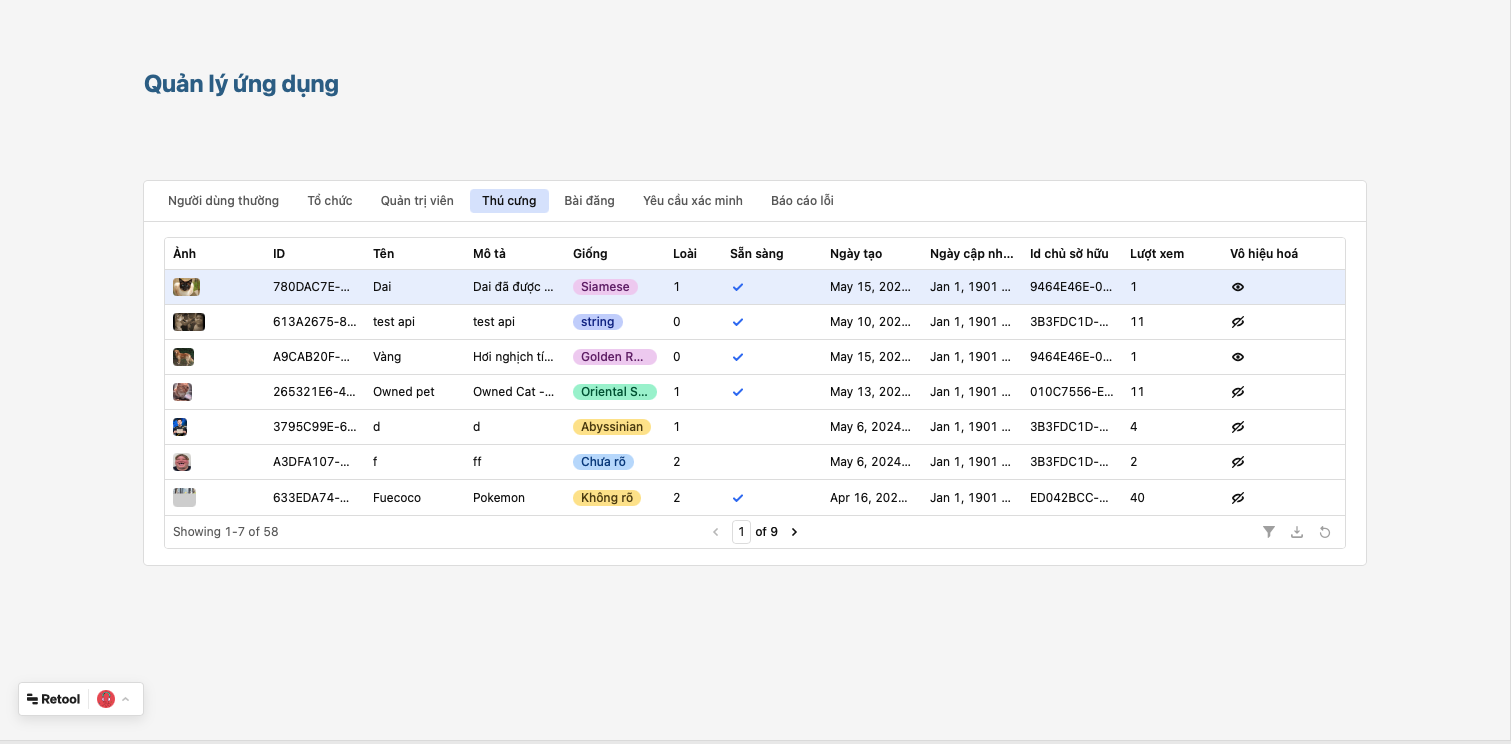
\includegraphics[width=0.7\textwidth]{Figures/UI/control_bo_ui.png}
\caption{Control page for managing data records}
\end{figure}

\newpage
\section{Database design}

\subsection{Conceptual design}

The conceptual design phase of the project is a pivotal stage in the development lifecycle, focused on establishing a comprehensive understanding of the system's structure and relationships.
\\
In \textit{Figure 3.18}, all entities and relationships are presented. Note that all attributes are excluded to enhance visualization and maintain a clear focus on the primary components shaping the system. These attributes will be shown in the physical design section.

\begin{figure}[H]
    \centering
    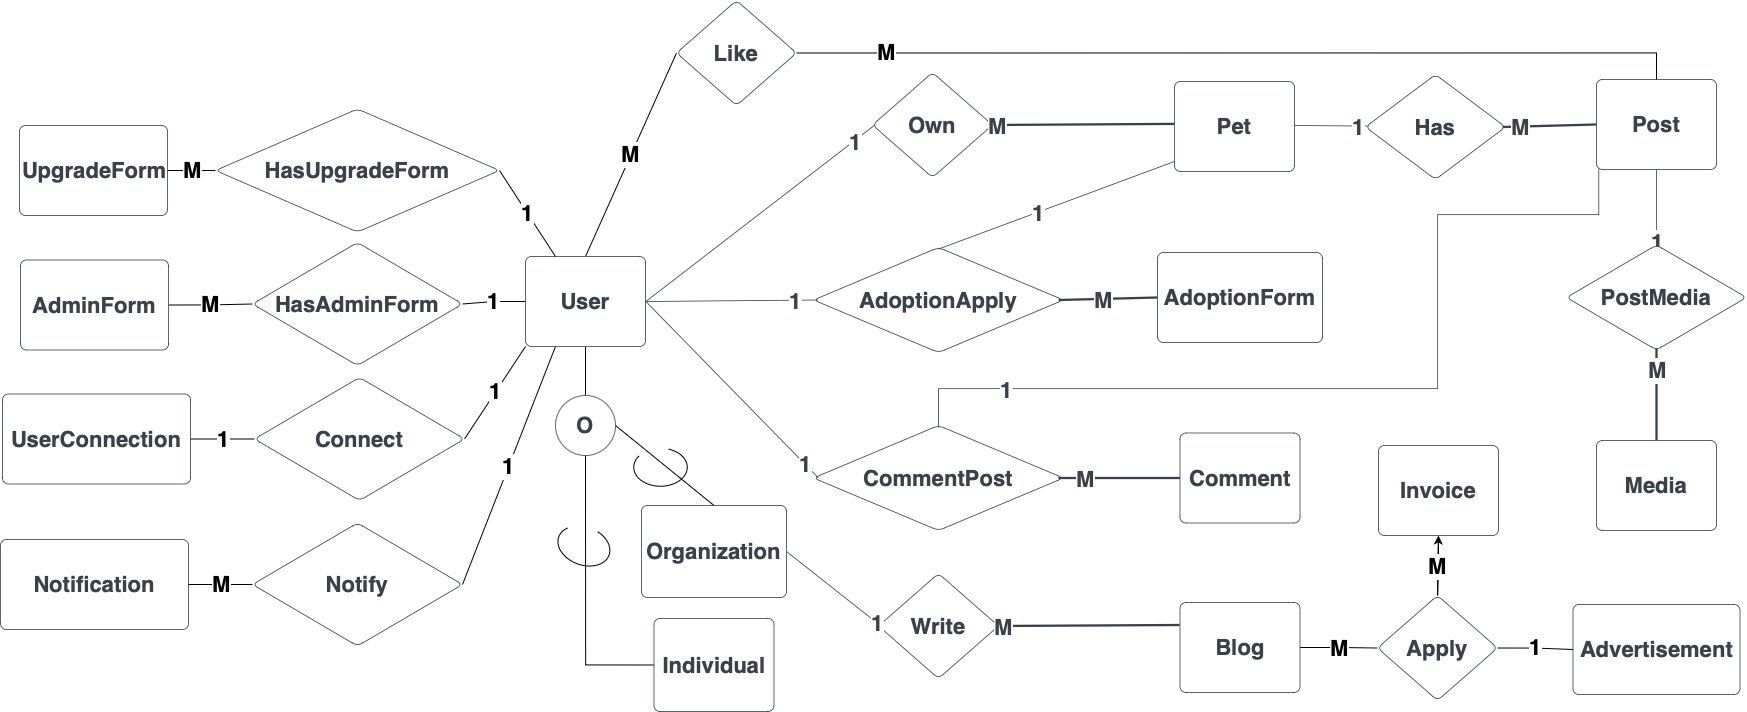
\includegraphics[angle=-90,width=0.4\textwidth]{Figures/DatabaseDesign/Entities-ERD.png}
    \caption{Entity-Relationship diagram}
\end{figure}
\clearpage

\subsection{Relational Design}

In the relational design phase, we use the relational mapping approach
to translate the abstract concepts from the Entity-Relationship Diagram
(ERD) into a concrete relational schema. Through the mapping process,
each entity, along with its attributes and relationships, is
systematically transformed into tables with defined fields and
corresponding constraints in \emph{Figure 3.19}.

\begin {figure}[H]
\centering
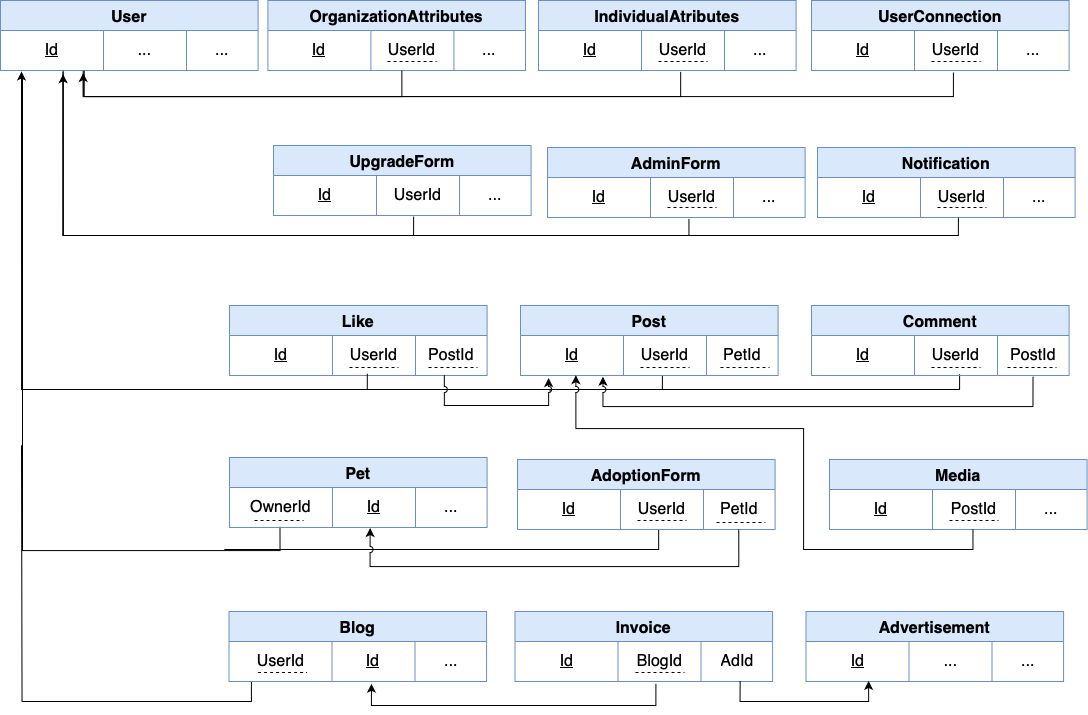
\includegraphics[width=0.9\textwidth]{Figures/DatabaseDesign/Entities-Mapping.png}
\caption{Relational schema}
\end{figure}

\emph{Figure 3.19}, the attributes are not presented fully to ensure a clear visualization of the diagram. In the relational mapping process, we implement a simplified technique for the 3-way relationship where the mandatory entity will take the primary key of the two optional entities as its foreign key, avoiding creating another table causes the schema to become unnecessarily complicated.

\subsection{Physical Design}

In this phase, the conceptual transforms into the tangible, as we build the actual blueprint that mirrors the intricacies of the adoption process in real life. The Relational Schema serves as our guidepost, detailing the tables, and relationships that will form the foundation of the physical database. \textit{Figure 3.20 and 3.21} below translates abstract entities and relationships into concrete data types and optimizes storage structures.

\begin {figure}[H]
\centering
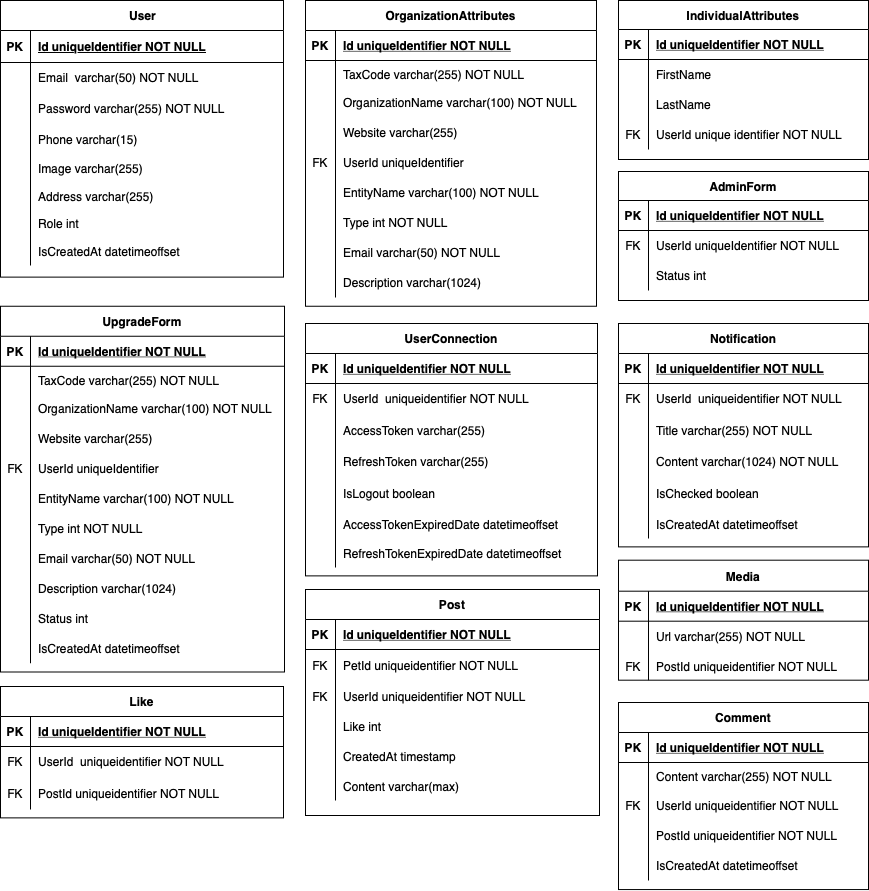
\includegraphics[width=0.8\textwidth]{Figures/DatabaseDesign/Entities-Physical_1.png}
\caption{Physical design}
\end{figure}

\begin {figure}[H]
\centering
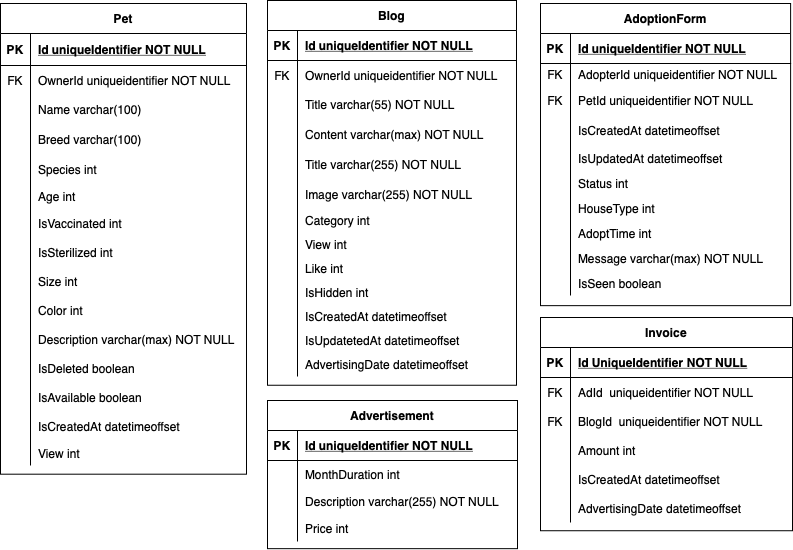
\includegraphics[width=0.8\textwidth]{Figures/DatabaseDesign/Entities-Physical_2.png}
\caption{Physical design (cont)}
\end{figure}





\chapter{DEVELOPMENT TECHNOLOGIES}

\section{Front-end}


In this section, we will dive into Next.js and Tailwind CSS. Next.js is
a React framework with features like server-side rendering, while
Tailwind CSS is a utility-first framework for streamlined styling
through pre-designed classes. These tools play a key role in creating
efficient and scalable front-end experiences.


\subsection{NextJS}

Next.js, a robust React framework, tackles challenges in traditional
client-side rendering. It utilizes server-side rendering and static site
generation to address accessibility, security, page loading times, and
Search engine optimization (SEO) concerns. Popular in the React
ecosystem, Next.js optimizes the user experience by pre-rendering pages
on the server. Advantages include enhanced performance with server-side
rendering, seamless React integration for dynamic interfaces, static
site generation for optimal website performance, intuitive file
system-based routing, automatic code splitting, flexible styling
approaches, and compatibility with TypeScript for improved code quality.


\subsection{Tailwind CSS}

Tailwind CSS, a utility-first framework, transforms web styling by
providing an extensive set of classes directly within HTML. This
accelerates development by offering granular control over layout, color,
spacing, and more. Unlike traditional CSS, Tailwind\textquotesingle s
unique approach eliminates the need for external files, enabling
seamless customization and efficient creation of visually appealing and
responsive interfaces. Its utility-first approach minimizes unused CSS,
optimizing performance, and its low learning curve, active community,
and integration flexibility make it an efficient choice for building
well-styled and maintainable web applications.


\section{Back-end}

\subsection{ASP.NET core platform}

ASP.NET Core, an open-source framework, excels in developing modern,
cloud-enabled, and Internet-connected applications with cross-platform
compatibility. It supports various applications, including web apps,
IoT, and mobile backends, allowing developers to use preferred tools
across Windows, macOS, and Linux. Offering seamless deployment to both
cloud and on-premises environments, ASP.NET Core operates on the .NET
Core runtime, empowering developers to create robust, scalable
applications. It represents a leaner and more modular evolution from
ASP.NET 4.0, unifying web UI and APIs, emphasizing testability, and
introducing innovations like Blazor for C\# usage in the browser.
ASP.NET Core is versatile, open-source, supports gRPC, and offers
flexible hosting options, showcasing its adaptability and
community-driven focus.

\subsection{Entity Framework}

Entity Framework is an open-source Object-Relational Mapping (ORM)
framework by Microsoft for .NET applications, abstracting database
complexities through domain-specific classes. Operating at a higher
level of abstraction, it simplifies data-oriented application creation,
resulting in concise and productive code. Features include Entity Data
Model, LINQ queries, raw SQL execution, change tracking, transaction
management, built-in caching, concurrency control, and asynchronous
saving. It adheres to conventions-over-configuration programming and
provides migration commands for seamless database schema management,
making Entity Framework a robust tool for efficient database development
in .NET applications.


\subsection{MS SQL Server}

Microsoft SQL Server stands as a formidable relational database
management system (RDBMS) catering to a diverse range of applications in
corporate IT environments, including transaction processing, business
intelligence, and analytics. It holds a prominent position among the top
three database technologies, alongside Oracle Database and
IBM\textquotesingle s DB2. Operating on the standardized SQL programming
language, SQL Server empowers database administrators and IT
professionals to efficiently manage databases and query their data. The
system is intricately connected to Transact-SQL (T-SQL), a Microsoft
implementation of SQL that introduces proprietary programming
extensions, enhancing the functionality of the standard language. This
combination of robust features and integration with the widely-used SQL
language makes Microsoft SQL Server a key player in the database
technology landscape.


\subsection{Redis Cache}

Redis, an open-source in-memory data structure store, serves multiple
roles as a database, cache, message broker, and streaming engine. Its
versatility lies in supporting various data structures like strings,
hashes, lists, sets, sorted sets with range queries, bitmaps, hyperlogs,
geospatial indexes, and streams. Redis boasts built-in features such as
replication, Lua scripting, LRU (Least Recently Used) eviction,
transactions, and diverse levels of on-disk persistence. Additionally,
it ensures high availability through Redis Sentinel and automatic
partitioning with Redis Cluster. This makes Redis a robust and flexible
solution for handling real-time data storage, retrieval, and processing
in a wide range of applications.


\subsection{Elastic-search}

Elasticsearch is a key component in the Elastic Stack ecosystem, serving
as a distributed search and analytics engine. Alongside Logstash and
Beats, it collects, aggregates, and enriches data, while Kibana enables
interactive exploration and visualization. Elasticsearch excels in near
real-time search and analytics for diverse data types, offering
scalability and flexibility. Its applications range from adding search
functionality to apps and storing logs to employing machine learning and
processing genetic data for various research purposes.

\subsection{ImgBB}

ImgBB is a user-friendly image hosting and sharing service that allows users to upload and share images easily. It supports various image formats such as JPEG, PNG, and GIF, making it versatile for different types of visual content. ImgBB provides features like direct image links, BBCode, and HTML thumbnails, which are particularly useful for embedding images in forums, websites, and social media. The service also includes functionalities like image resizing and expiration settings, giving users control over how and for how long their images are displayed.


\subsection{Retool}

Retool is a rapid development platform for building internal software quickly and efficiently. It features a drag-and-drop interface for creating custom applications, supports integration with a wide range of databases and APIs, and allows for the incorporation of custom JavaScript. With Retool, users can easily combine data from multiple sources and implement complex functionalities without extensive coding. Its built-in permissions and access controls ensure data security, making Retool a valuable tool for enhancing internal workflows and productivity.


\chapter*{Conclusion}


%-	Danh mục TL tham khảo
%-	Phụ lục (nếu có)

% comment two lines and use manually.bbl bellow if manually

% \bibliographystyle{plain} % ieeetr
% \bibliography{refs}

\input{manually.bbl}

\end{document}
